\documentclass[aspectratio=169,11pt]{beamer}

\usepackage[utf8]{inputenc}
\usepackage[T1]{fontenc}
\usepackage{graphicx}
\usepackage{booktabs}
\usepackage{amsmath}
\usepackage{tikz}
\usepackage{array}
\usepackage{multicol}

\usetheme{default}
\usecolortheme{dove}
\usefonttheme{professionalfonts}

\definecolor{ntua_blue}{RGB}{0,40,85}
\setbeamercolor{title}{fg=ntua_blue}
\setbeamercolor{frametitle}{fg=ntua_blue}
\setbeamercolor{structure}{fg=ntua_blue}

\setbeamertemplate{navigation symbols}{}
\setbeamertemplate{footline}[frame number]

\begin{document}

\begin{frame}[plain]
    \vspace*{0.5cm}

    \begin{minipage}[t]{0.13\textwidth}
        \vspace{0pt}
        
\includegraphics[width=\textwidth]{figures/pyrforos.eps}
    \end{minipage}
    \hfill
    \begin{minipage}[t]{0.83\textwidth}
        \vspace{1em}
        \small
        National Technical University of Athens\\
        School of Electrical and Computer Engineering\\
        Division of Computer Science
    \end{minipage}

    \vfill

    \begin{center}
        \begin{beamercolorbox}[wd=\linewidth,sep=6pt,center]{title}
            {\usebeamerfont{title} Joint Thesis Presentation}
        \end{beamercolorbox}

        \vspace{2em}

        {\small
            \renewcommand{\arraystretch}{1.1}%
            \begin{tabular}{@{}l@{\hspace{0.8em}}>{\raggedright\arraybackslash}p{0.65\linewidth}@{}}
                \textbf{Georgios Angelis}        & \textit{Applied Machine Learning in Distributed and Dynamic Environments} \\
                \textbf{Georgios Kyriakopoulos}  & \textit{Continuous Machine Learning for Cooperative, Connected and Automated Mobility applications} \\
                \textbf{Serafeim Tzelepis}       & \textit{Machine Learning under Concept Drift} \\
            \end{tabular}
        }
    \end{center}

    \vspace{2em}

    \begin{minipage}[b]{0.55\textwidth}
        \raggedright
        \small
        \textbf{Supervisor:} Professor Panayiotis Tsanakas
    \end{minipage}
    \hfill
    \begin{minipage}[b]{0.40\textwidth}
        \raggedleft
        \small
        30 October 2025
    \end{minipage}

    \vspace*{0.5cm}
\end{frame}

\begin{frame}[plain]{Presentation Outline}
    \tableofcontents
\end{frame}

\section{Introduction}

\begin{frame}{The Challenge}

    \textbf{Motivation}

    Machine Learning models in real-world settings degrade over time as data distributions shift, a phenomenon known as \textbf{Concept Drift}.

    \bigskip
    \textbf{Problem Statement}

    In urban mobility environments traffic conditions, weather, or roadworks alter traffic patterns.
    Static models cannot sustain accuracy under these evolving conditions.

    \bigskip
    \textbf{Solution}

    Develop a unified \textbf{urban mobility simulation platform} with real time monitoring, automated drift detection and adaptation.

\end{frame}

\begin{frame}{Platform Positioning}

    \textbf{Current Landscape}

    \begin{itemize}
        \item MLOps tools mostly \textbf{monitor/alert}, while adaptation is \textbf{manual}.
        \item Drift detectors are typically \textbf{task-specific} and \textbf{hand-tuned}, leading to inconsistent behavior across models.
    \end{itemize}

    \bigskip

    \textbf{Gap for Urban Mobility Platforms}

    \begin{itemize}
        \item Need a solution that offers \textbf{end-to-end} handling of \textbf{drift detection} and \textbf{adaptation}.
        \item Need a \textbf{lightweight, task-agnostic} service that works across models without tuning each detector.
    \end{itemize}

\end{frame}

\begin{frame}{Contributions}

    \begin{itemize}
        \item \textbf{SUMO Synthetic Dataset} including a scenario with concept drift, publicly available on Zenodo
            \medskip
        \item Three \textbf{Machine Learning models}:
            \medskip
            \begin{itemize}
                \item Estimated Time of Arrival
                    \medskip
                \item Fuel Consumption
                    \medskip
                \item Number of Stops
            \end{itemize}
            \medskip
        \item \textbf{Urban Mobility Simulation Platform} with complete automated drift lifecycle managment
    \end{itemize}

\end{frame}

\begin{frame}{Simulation Story}
    \begin{center}
        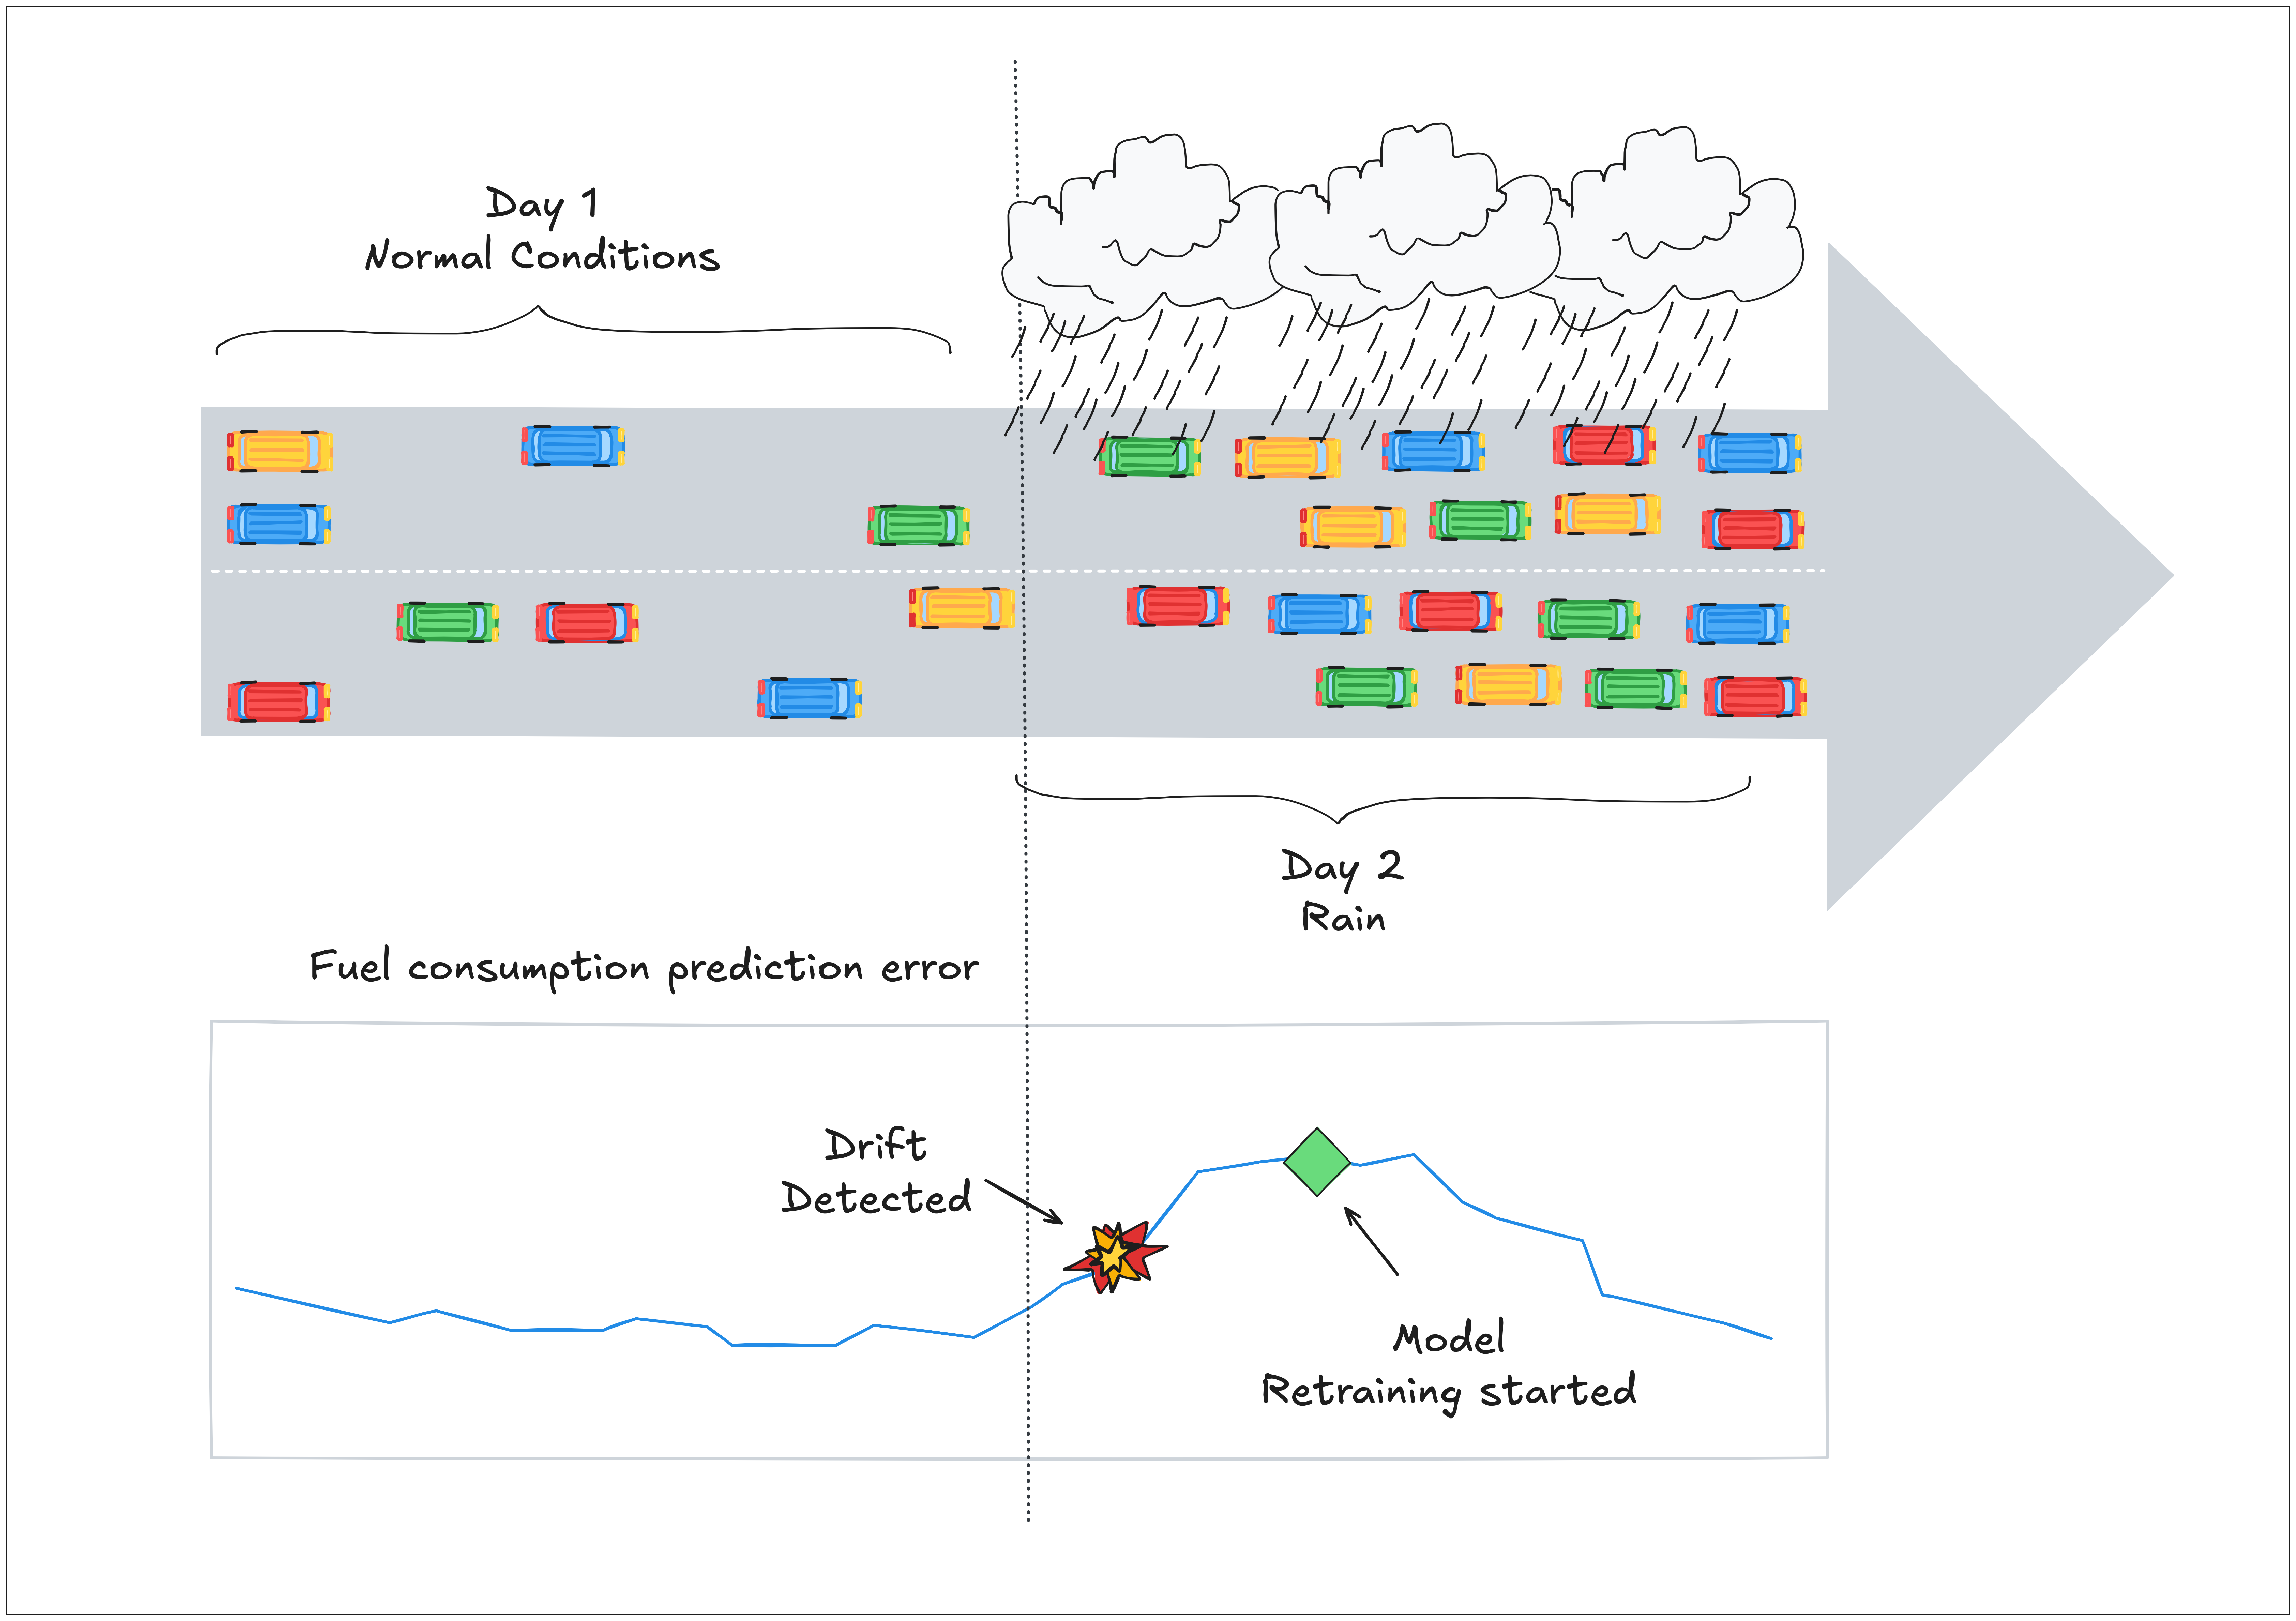
\includegraphics[width=0.55\textwidth]{figures/simulation-story.png}
    \end{center}

    \begin{itemize}
        \item Two-day simulation (10h/day): Normal $\rightarrow$ Rain conditions
        \item Drift detected $\rightarrow$  triggers drift adaptation
    \end{itemize}
\end{frame}

\section{Concept Drift}

\begin{frame}{Concept Drift — Definition \& Types}

    \textbf{Definition}
    \[
        P_t(Y\,|\,X)\;\neq\;P_{t+\Delta t}(Y\,|\,X)
    \]
    \small Change over time in the relationship (mapping) between inputs $X$ and target $Y$.\normalsize

    \vspace{0.6em}
    \textbf{Types (with urban mobility examples)}
    \begin{itemize}
        \item \textbf{Sudden / Abrupt}: heavy rain or road closure → instant speed/stop change.
        \item \textbf{Gradual}: rush hour forms and dissolves over time.
        \item \textbf{Recurring / Seasonal}: tourist season repeats yearly traffic patterns.
        \item \textbf{Incremental}: new roads/signals slowly reshape traffic flow.
    \end{itemize}

\end{frame}

\section{Dataset Generation}

\begin{frame}{Study Area \& Scenarios}
    \begin{itemize}
        \item \textbf{Tooling:} SUMO (microscopic), headless scripts, reproducible seeds/config.
            \medskip
        \item \textbf{Study area:} Central Athens (dense and urban area) $\approx 2.5 \text{ km} \times 1.5 \text{ km}$
            \medskip
        \item \textbf{Scenarios:}
            \medskip
            \begin{itemize}
                \item \textbf{Train:} Baseline conditions for model training.
                    \medskip
                \item \textbf{Test:} Baseline conditions for model evaluation.
                    \medskip
                \item \textbf{Rain:} Rain conditions with reduced lane friction for drift evaluation.
            \end{itemize}
    \end{itemize}
\end{frame}

\begin{frame}{Traffic Demand \& Trip Generation}
    \begin{itemize}
        \item \textbf{Horizon:} {08:00--18:00} (10 hours).
            \medskip
        \item \textbf{Traffic Demand:} Realistic hourly profile (morning and evening peak, midday decline) with light Gaussian noise for variability.
            \medskip
        \item \textbf{Trip creation:} \texttt{randomTrips.py} with \textbf{distinct seeds} per scenario; passenger cars focus (reduced heterogeneity).
            \medskip
        \item \textbf{Outputs:} timestep, id, x, y, speed, lane, odometer, fuel, waiting
    \end{itemize}
\end{frame}

\begin{frame}{Drift Mechanism: Why Rain?}
    \begin{itemize}
        \item \textbf{Alternatives considered:} Lane closures (rerouting needed), edge closures (irreversible network changes), driving behavior tweaks (weak and unrealistic).
            \medskip
        \item \textbf{Chosen mechanism:} Decrease lane friction from 1.0 to 0.4 (physics-grounded, no rerouting bias, no topology changes, global effect).
            \medskip
        \item \textbf{Takeaway:} Strong but non-catastrophic shift $\Rightarrow$ ideal for abrupt drift detection without breaking comparability.
            \medskip
        \item \textbf{Rain vs.\ Test:}
            \medskip
            \begin{itemize}
                \item Average speed \textbf{-13.68\%} (\(\approx\) 29.81 $\to$ 25.74 km/h)
                    \medskip
                \item Trip duration \textbf{+16.74\%} (\(\approx\) 211.58 $\to$ 247.00 s)
            \end{itemize}
    \end{itemize}
\end{frame}

\section{Machine Learning Research}

\begin{frame}{ETA Task and Literature Review}
    \begin{itemize}
        \item \textbf{Why ETA matters:} reliable ETAs drive routing, signal timing, parking management, and user trust in CCAM.
        \item \textbf{Drift challenge:} non-stationary urban traffic with the \emph{rain} scenario inducing a measurable shift (speeds, waiting, duration).
    \end{itemize}

    \bigskip
    \begin{itemize}
        \item \textbf{Classical time series:} ARIMAs are limited under nonlinear or context-rich traffic.
        \item \textbf{Deep sequence models:} RNN/LSTM/CNN/Transformers to capture local or global patterns and GNNs to propagate congestion with strong production results.
        \item \textbf{Gradient boosting:} competitive with tabular data and engineered features, and fast to retrain under drift.
    \end{itemize}
\end{frame}

\begin{frame}{Target, Trip Features, and Setup}
    \begin{itemize}
        \item \textbf{Prediction target:} Trip duration in seconds (ETA).
            \medskip
        \item \textbf{Trip features:} \texttt{time\_start}, \texttt{source\_x}, \texttt{source\_y}, \texttt{destination\_x}, \texttt{destination\_y}, \texttt{distance}
            \medskip
        \item \textbf{Evaluation setup:} 5-fold \textbf{stratified} CV on train (by target) with MAE (s), MAPE (\%) and training time (s) as metrics.
            \medskip
        \item \textbf{Baseline models:} Linear Regression, LightGBM, XGBoost, CatBoost.
    \end{itemize}
\end{frame}

\begin{frame}{Transforms, Feature Engineering and Tuning}
    \textbf{Transformations}
    \begin{itemize}
        \item Tried: \texttt{log(1+x)} on distance, standard scaling, target log/Box-Cox/quantile.
        \item Result: no consistent gain over GBDT baseline, as expected for tree-based models.
    \end{itemize}

    \textbf{Feature engineering and selection}
    \begin{itemize}
        \item Temporal (hour/peaks), Spatial (distance/bearing/centrality/detours), Fourier positional encodings, Cell grid, Clusters KMeans, PCA source/destination.
        \item \textbf{Top signals:} \texttt{distance}, \texttt{euclidean\_distance}, \texttt{x\_center}, \texttt{y\_center}, \texttt{detour\_length}, \texttt{time\_start}, clusters, PCA components.
    \end{itemize}

    \textbf{Tuning}
    \begin{itemize}
        \item One broad and one focused Optuna search, with the objective of minimizing MAE.
        \item \textbf{LightGBM} selected with MAE \textbf{26.51 s}, MAPE \textbf{12.77\%} and training time \textbf{2.95 s}.
    \end{itemize}
\end{frame}

\begin{frame}{Fuel Consumption Prediction Task \& Literature Review}
    \begin{itemize}
        \item \textbf{Task framing:} Predict per-trip fuel from SUMO-derived data.
        \item \textbf{Drift \& adaptation:} Rain induces distribution shift; retraining restores accuracy and supports mobility decision tools.
        \item \textbf{Modeling landscape:} Tree-based ensemble learners excel on structured, tabular vehicle-feature data for predicting fuel efficiency (Yoo et al., 2025), Sequence models—e.g., FuelNet (Wang et al., 2020)—learn speed-/acceleration-sequence patterns for fuel-consumption prediction, Comprehensive feature engineering across vehicle attributes strengthens ensemble learners’ predictive reliability (Yoo et al., 2025).
    \end{itemize}
\end{frame}

\begin{frame}{Data Preprocessing Pipeline}

    \textbf{SUMO Traffic Simulation:} Athens central network, synthetic FCD data

    \vspace{0.5em}
    \begin{columns}[T]
        \column{0.55\textwidth}
        \textbf{Pipeline Steps:}
        \begin{enumerate}
            \item \textbf{Data Generation:} SUMO microscopic simulation
            \item \textbf{Trip Aggregation:} Timestep $\rightarrow$ trip-level
            \item \textbf{Feature Engineering:} Temporal, spatial, distance
            \item \textbf{Spatial Clustering:} K-means (k=10) for OD pairs
            \item \textbf{Target Transform:} Log(1+x) for normalization
        \end{enumerate}

        \column{0.42\textwidth}
        \begin{center}
            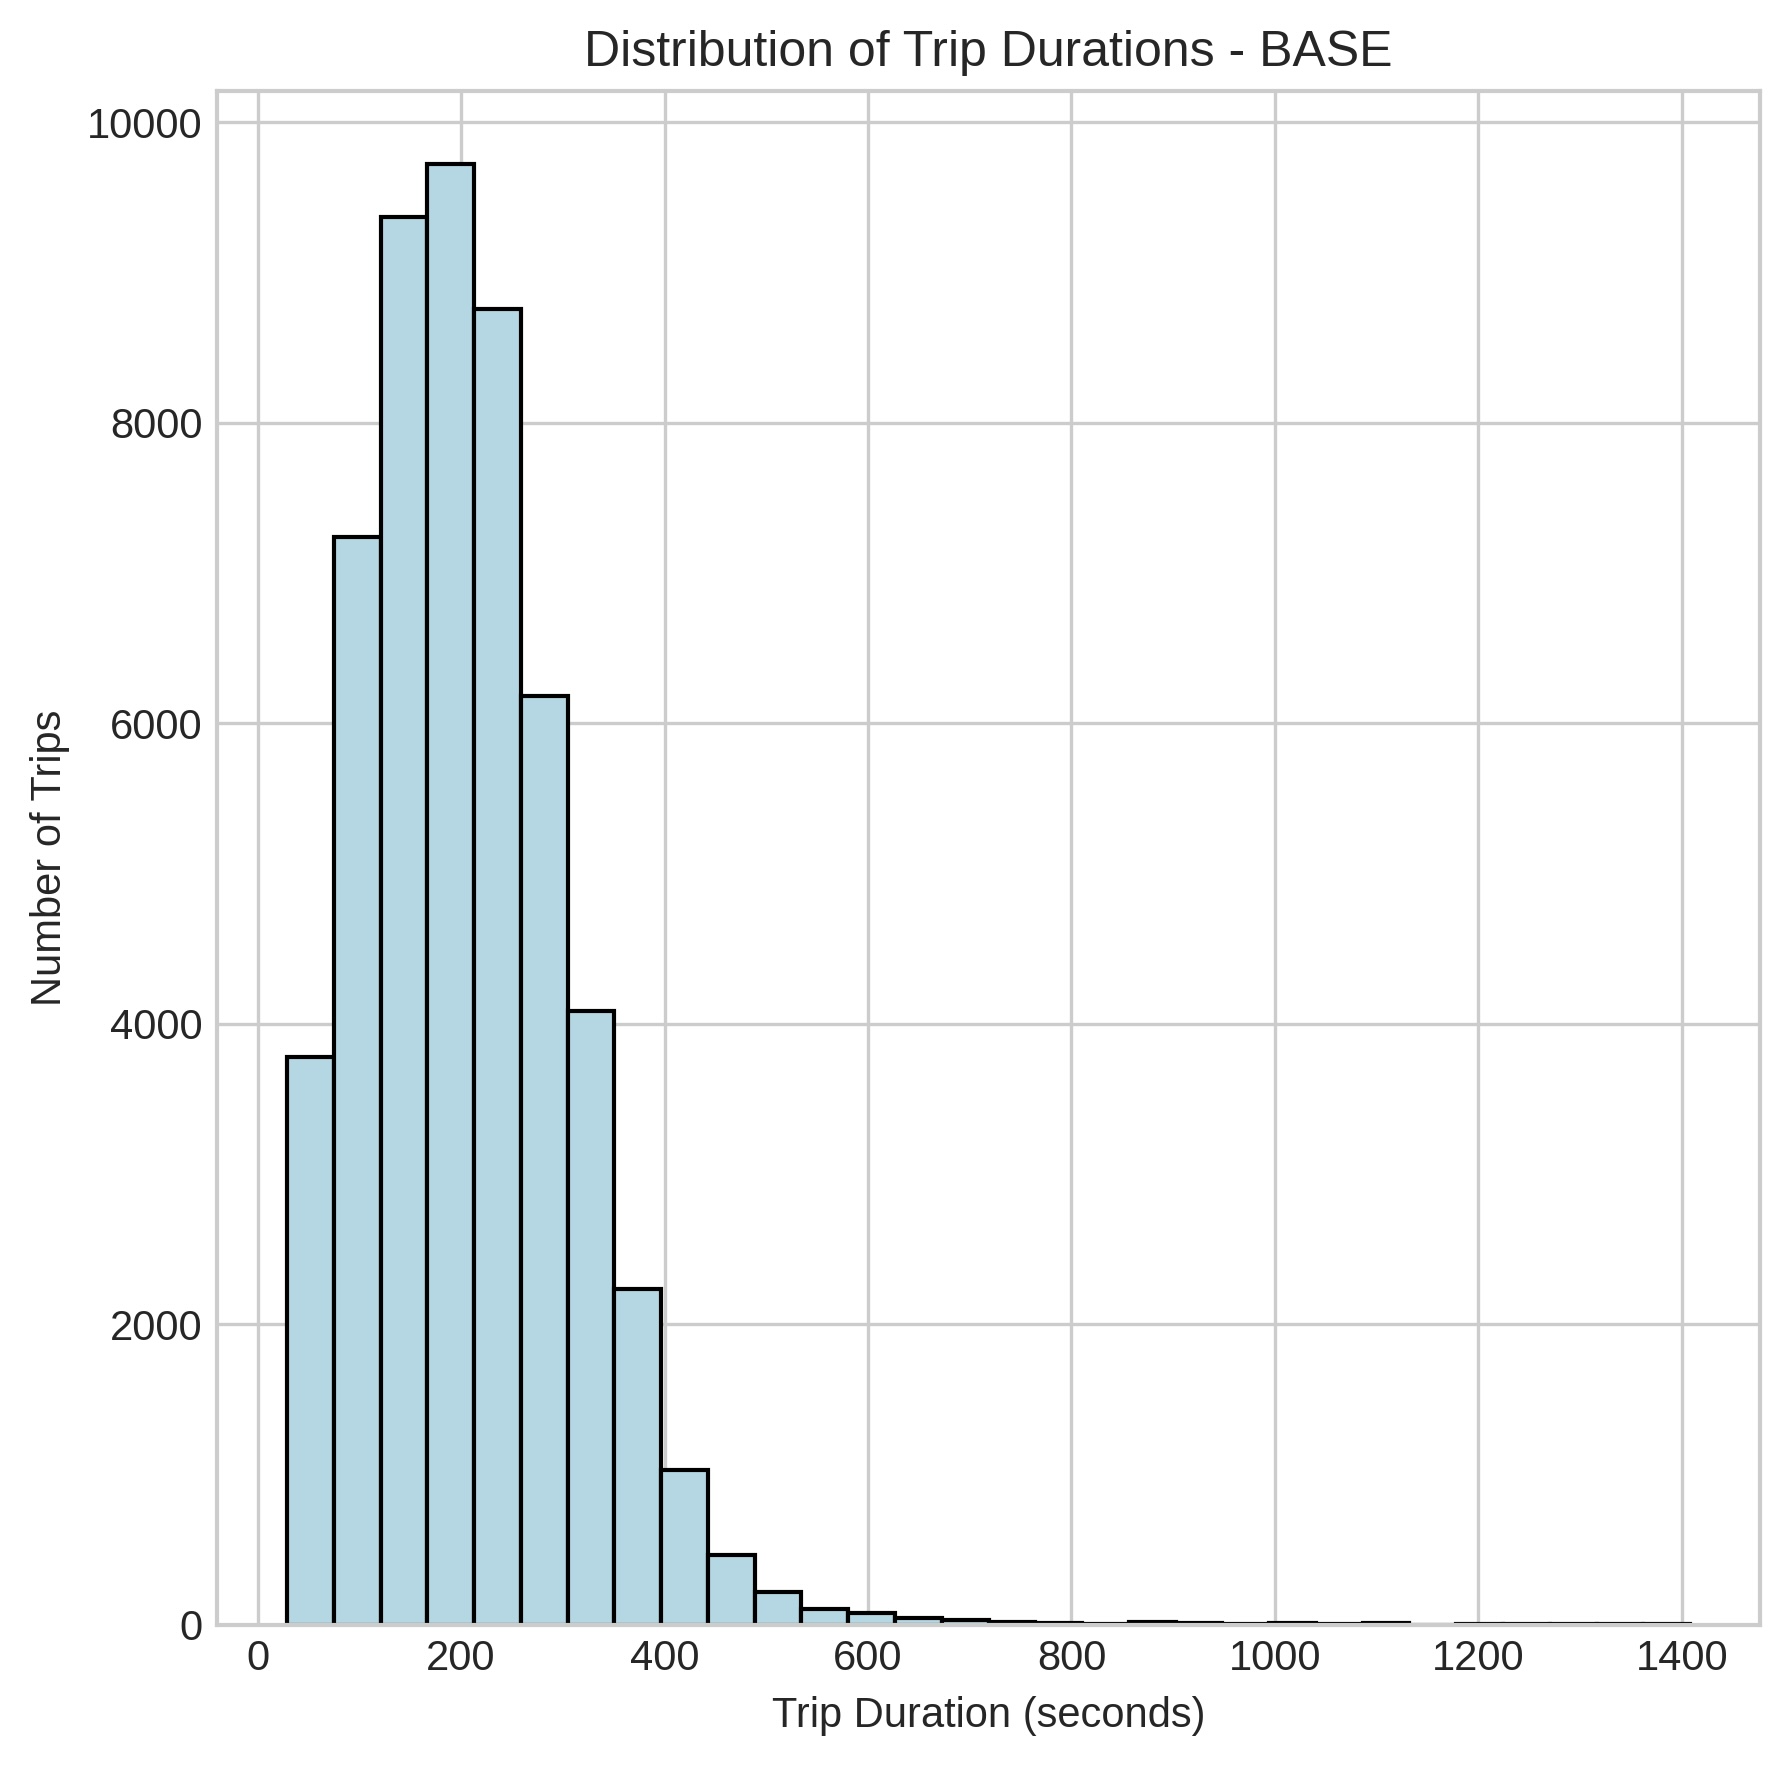
\includegraphics[width=0.7\textwidth]{figures/fuel-trips.png}\\
            {\footnotesize Trip characteristics distribution}
        \end{center}
    \end{columns}

    \vspace{0.3em}
    \textbf{Final Dataset:} 53,441 training trips, 29 engineered features
\end{frame}

\begin{frame}{Exploratory Data Analysis \& Feature Relationships}
    \begin{columns}[c,onlytextwidth]
        \column{0.52\textwidth}
        \centering
        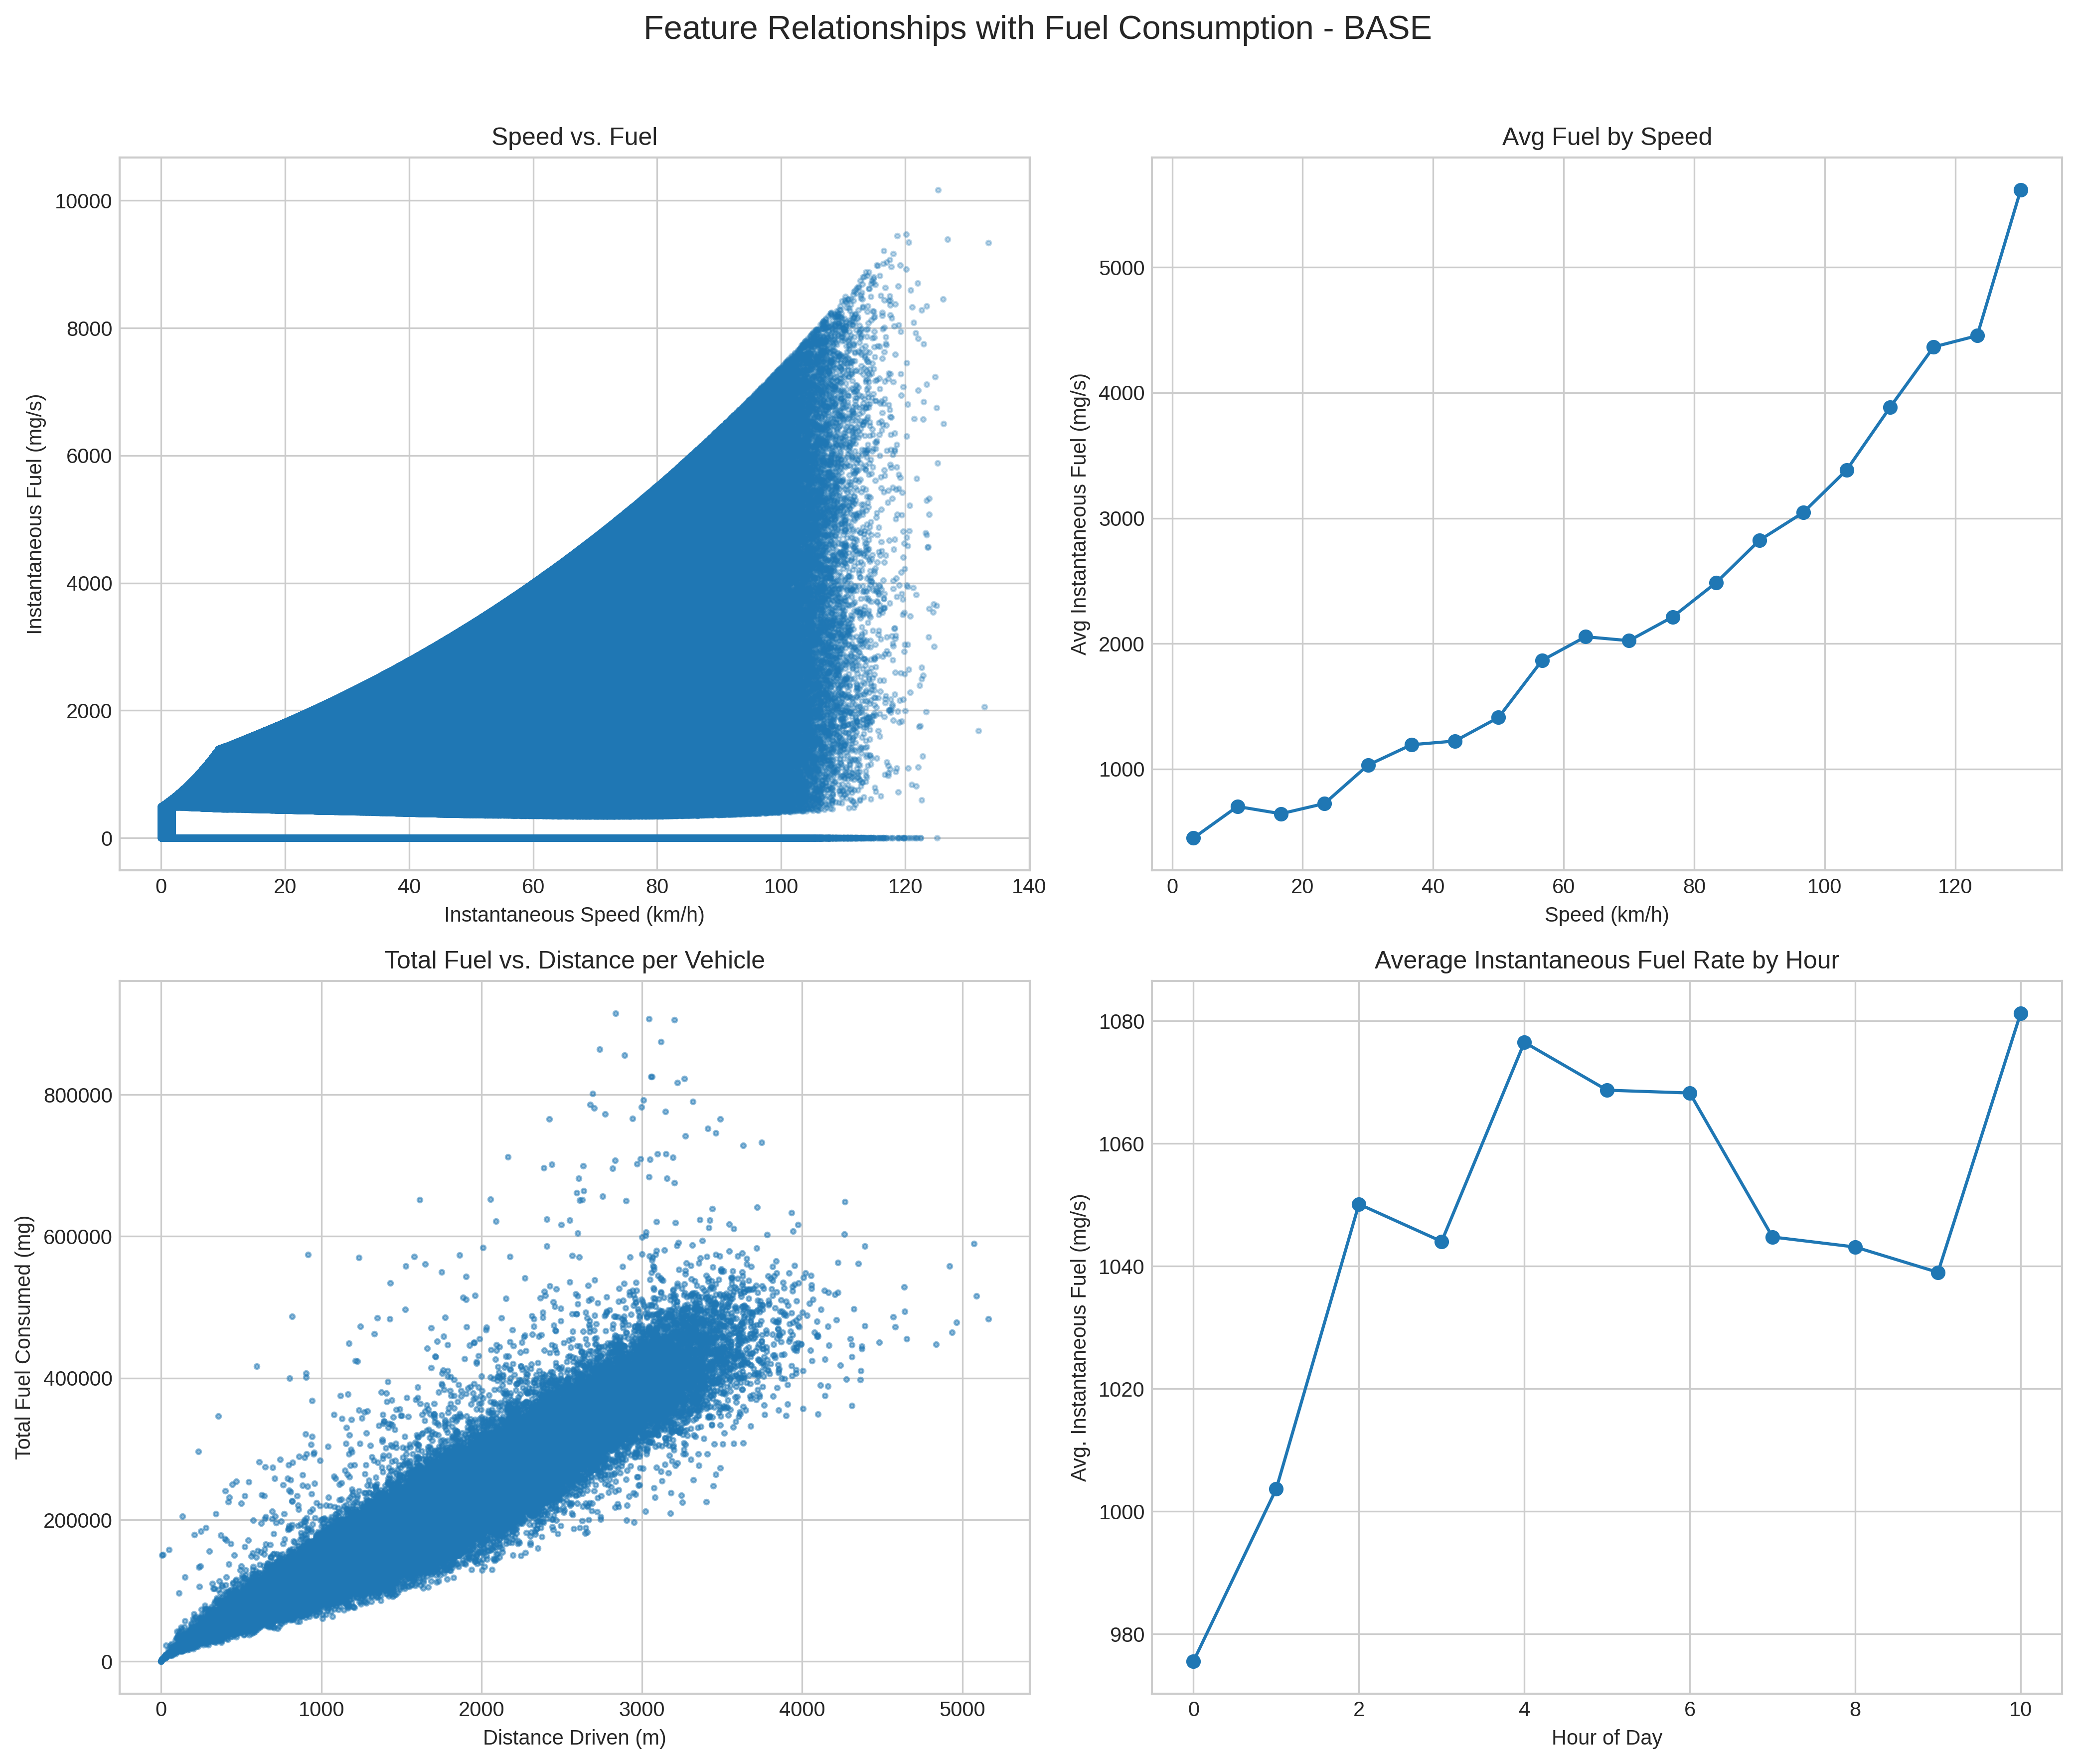
\includegraphics[width=\linewidth]{figures/fuel-features.png}

        \column{0.48\textwidth}
        \vspace{-0.5em}
        \begin{itemize}
            \item Non-linear speed-fuel relationship
            \item Strong linear correlation between distance and total fuel consumption
            \item Temporal variations in hourly fuel consumption patterns
        \end{itemize}
    \end{columns}
\end{frame}

\begin{frame}{Machine Learning Model Selection \& Performance}

    \textbf{Model Selection:} XGBoost with log-transformed targets

    \vspace{0.5em}
    \begin{columns}[c]
        \column{0.55\textwidth}
        \begin{table}
            \centering
            \small
            \begin{tabular}{lccc}
                \toprule
                \textbf{Dataset} & \textbf{MAE} & \textbf{R²} & \textbf{MAPE} \\
                \midrule
                Test (Base) & 20,867 mg & 0.860 & 9.61\% \\
                Rain (Drift) & 22,001 mg & 0.813 & 9.54\% \\
                \midrule
                \multicolumn{4}{l}{\textbf{Degradation:} +5.43\% MAE} \\
                \multicolumn{4}{l}{\textit{Retrained Model:} -2.5\% MAE} \\
                \bottomrule
            \end{tabular}
        \end{table}

        \vspace{0.3em}
        \textbf{Why XGBoost?}
        \begin{itemize}
            \item Best performance among models supporting incremental learning
            \item Hyperparameter tuning: GridSearch + TimeSeriesSplit (3-fold)
        \end{itemize}

        \column{0.42\textwidth}
        \textbf{Key Results:}
        \begin{itemize}
            \item Minimal degradation under drift
            \item Effective incremental adaptation
            \item Maintains $<$ 10\% MAPE
        \end{itemize}

        \vspace{0.5em}
        \textbf{8 Models Evaluated:}
        {\footnotesize XGBoost, HistGB, RandomForest, ExtraTrees, AdaBoost, LinearReg, KNN, MLP}
    \end{columns}

\end{frame}

\begin{frame}{Number of Stops Prediction}

    \textbf{Problem}
    \begin{itemize}
        \item Predict the \textbf{number of full stops} a vehicle makes during a trip or segment.
        \item Formulated as a \textbf{regression} task on trip-level features.
    \end{itemize}

    \vspace{0.6em}
    \textbf{Why it matters}
    \begin{itemize}
        \item \textbf{Route optimization}: fewer expected stops can guide route choice.
        \item \textbf{Traffic-signal planning}: stop intensity highlights phases/intersections to retime.
        \item \textbf{Safety \& comfort}: excessive stop-go patterns indicate unstable traffic regimes.
    \end{itemize}
\end{frame}
\begin{frame}{Feature Engineering - Spatial \& Route Design}

    \textbf{Spatial representation (K-Means, $k{=}7$)}
    \begin{itemize}
        \item Source/Destination \textbf{cluster IDs} (one-hot for src/dst).
        \item \textbf{Distance to each cluster center} for src/dst and \textbf{distance to city center}.
    \end{itemize}

    \vspace{0.6em}
    \textbf{Zone priors (target encoding)}
    \begin{itemize}
        \item \textbf{Mean stops per cluster} for src/dst clusters (proxy for historical stop rates).
    \end{itemize}

    \vspace{0.6em}
    \textbf{Temporal context}
    \begin{itemize}
        \item Departure time, time-of-day encoding, within-day sequence index.
    \end{itemize}

    \vspace{0.6em}
    \textbf{Route complexity}
    \begin{itemize}
        \item Total segments; share of unique segments (turns/intersections); segment reuse ratio (loops/backtracking)
    \end{itemize}
\end{frame}
\begin{frame}{Models \& Configuration Space}

    \textbf{Model families}
    \begin{itemize}
        \item Baseline: Linear Regression
        \item Tree ensembles: \textbf{XGBoost}, LightGBM, CatBoost
        \item Neural: MLP
    \end{itemize}

    \vspace{0.6em}
    \textbf{Configuration toggles (checked for \emph{each} model)}
    \begin{itemize}
        \item \textbf{Scaling}: none \ / \ standardization
        \item \textbf{Target}: raw \ / \ \(\log(1+\text{stops})\)
        \item \textbf{Features}: route features on/off, spatial features on/off
        \item \textbf{Feature pruning}: feature importance based pruning on/off
    \end{itemize}

    \vspace{0.6em}
    \textbf{Tuning \& selection}
    \begin{itemize}
        \item CV (cross validation) evalutation for all the possible configuration combos and parameters (per model)
        \item Primary metric: \textbf{MAE}, also support: \(R^2\) and \(RMSE\)
    \end{itemize}

\end{frame}
\begin{frame}{Final Model Selection}
    \vspace{0.6em}
    \textbf{Outcome}
    \begin{itemize}
        \item Primary metric: \textbf{MAE}, support: \(R^2\) for distribution sanity checks
        \item \textbf{XGBoost} achieved the lowest CV MAE consistently across configurations.
        \item Chosen for its accuracy and \textbf{incremental retraining} compatibility with the drift pipeline.
    \end{itemize}

\end{frame}

\section{Platform Implementation}

\begin{frame}{Platform Concept Evolution}
    \begin{center}
        \textbf{Early Conceptualization (March 2025)}\\[0.3em]
        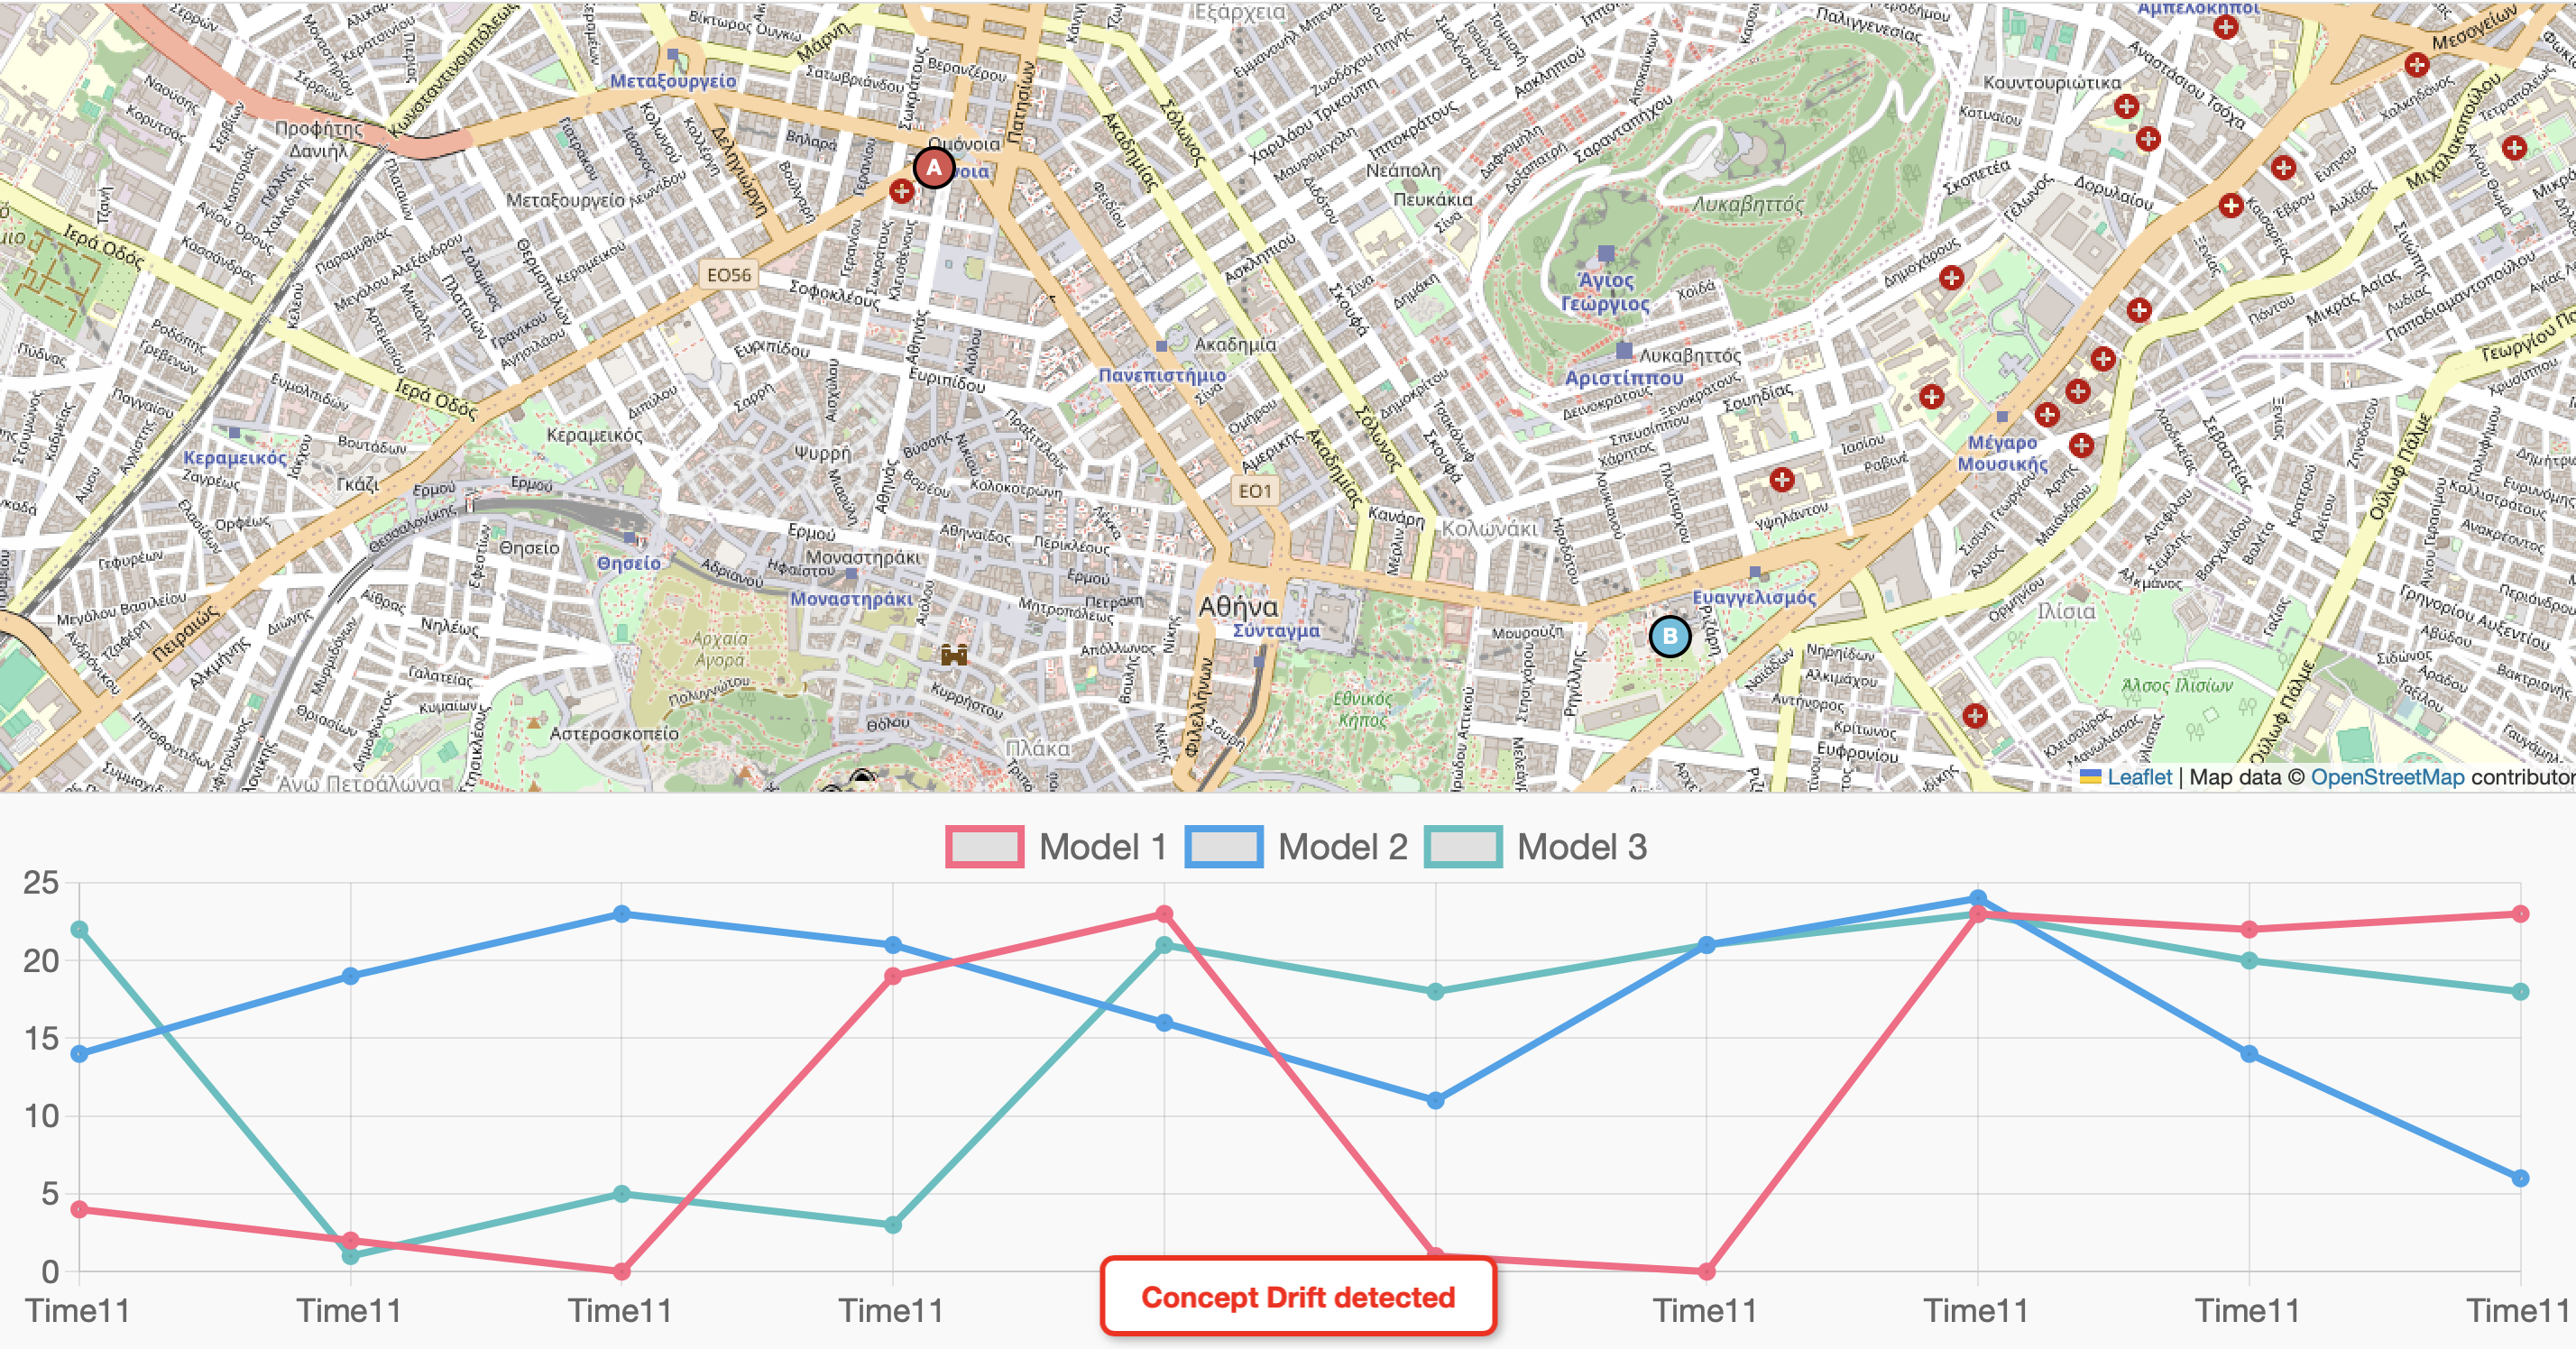
\includegraphics[width=0.6\textwidth]{figures/early-conceptualization.png}
    \end{center}

    \begin{itemize}
        \item Initial vision: Multi-model monitoring with drift detection
        \item Athens traffic map visualization with performance tracking
        \item Time-series plots
    \end{itemize}
\end{frame}

\begin{frame}{Platform Prototype Refinement}
    \begin{center}
        \textbf{UI mockup (July 2025)}\\[0.3em]
        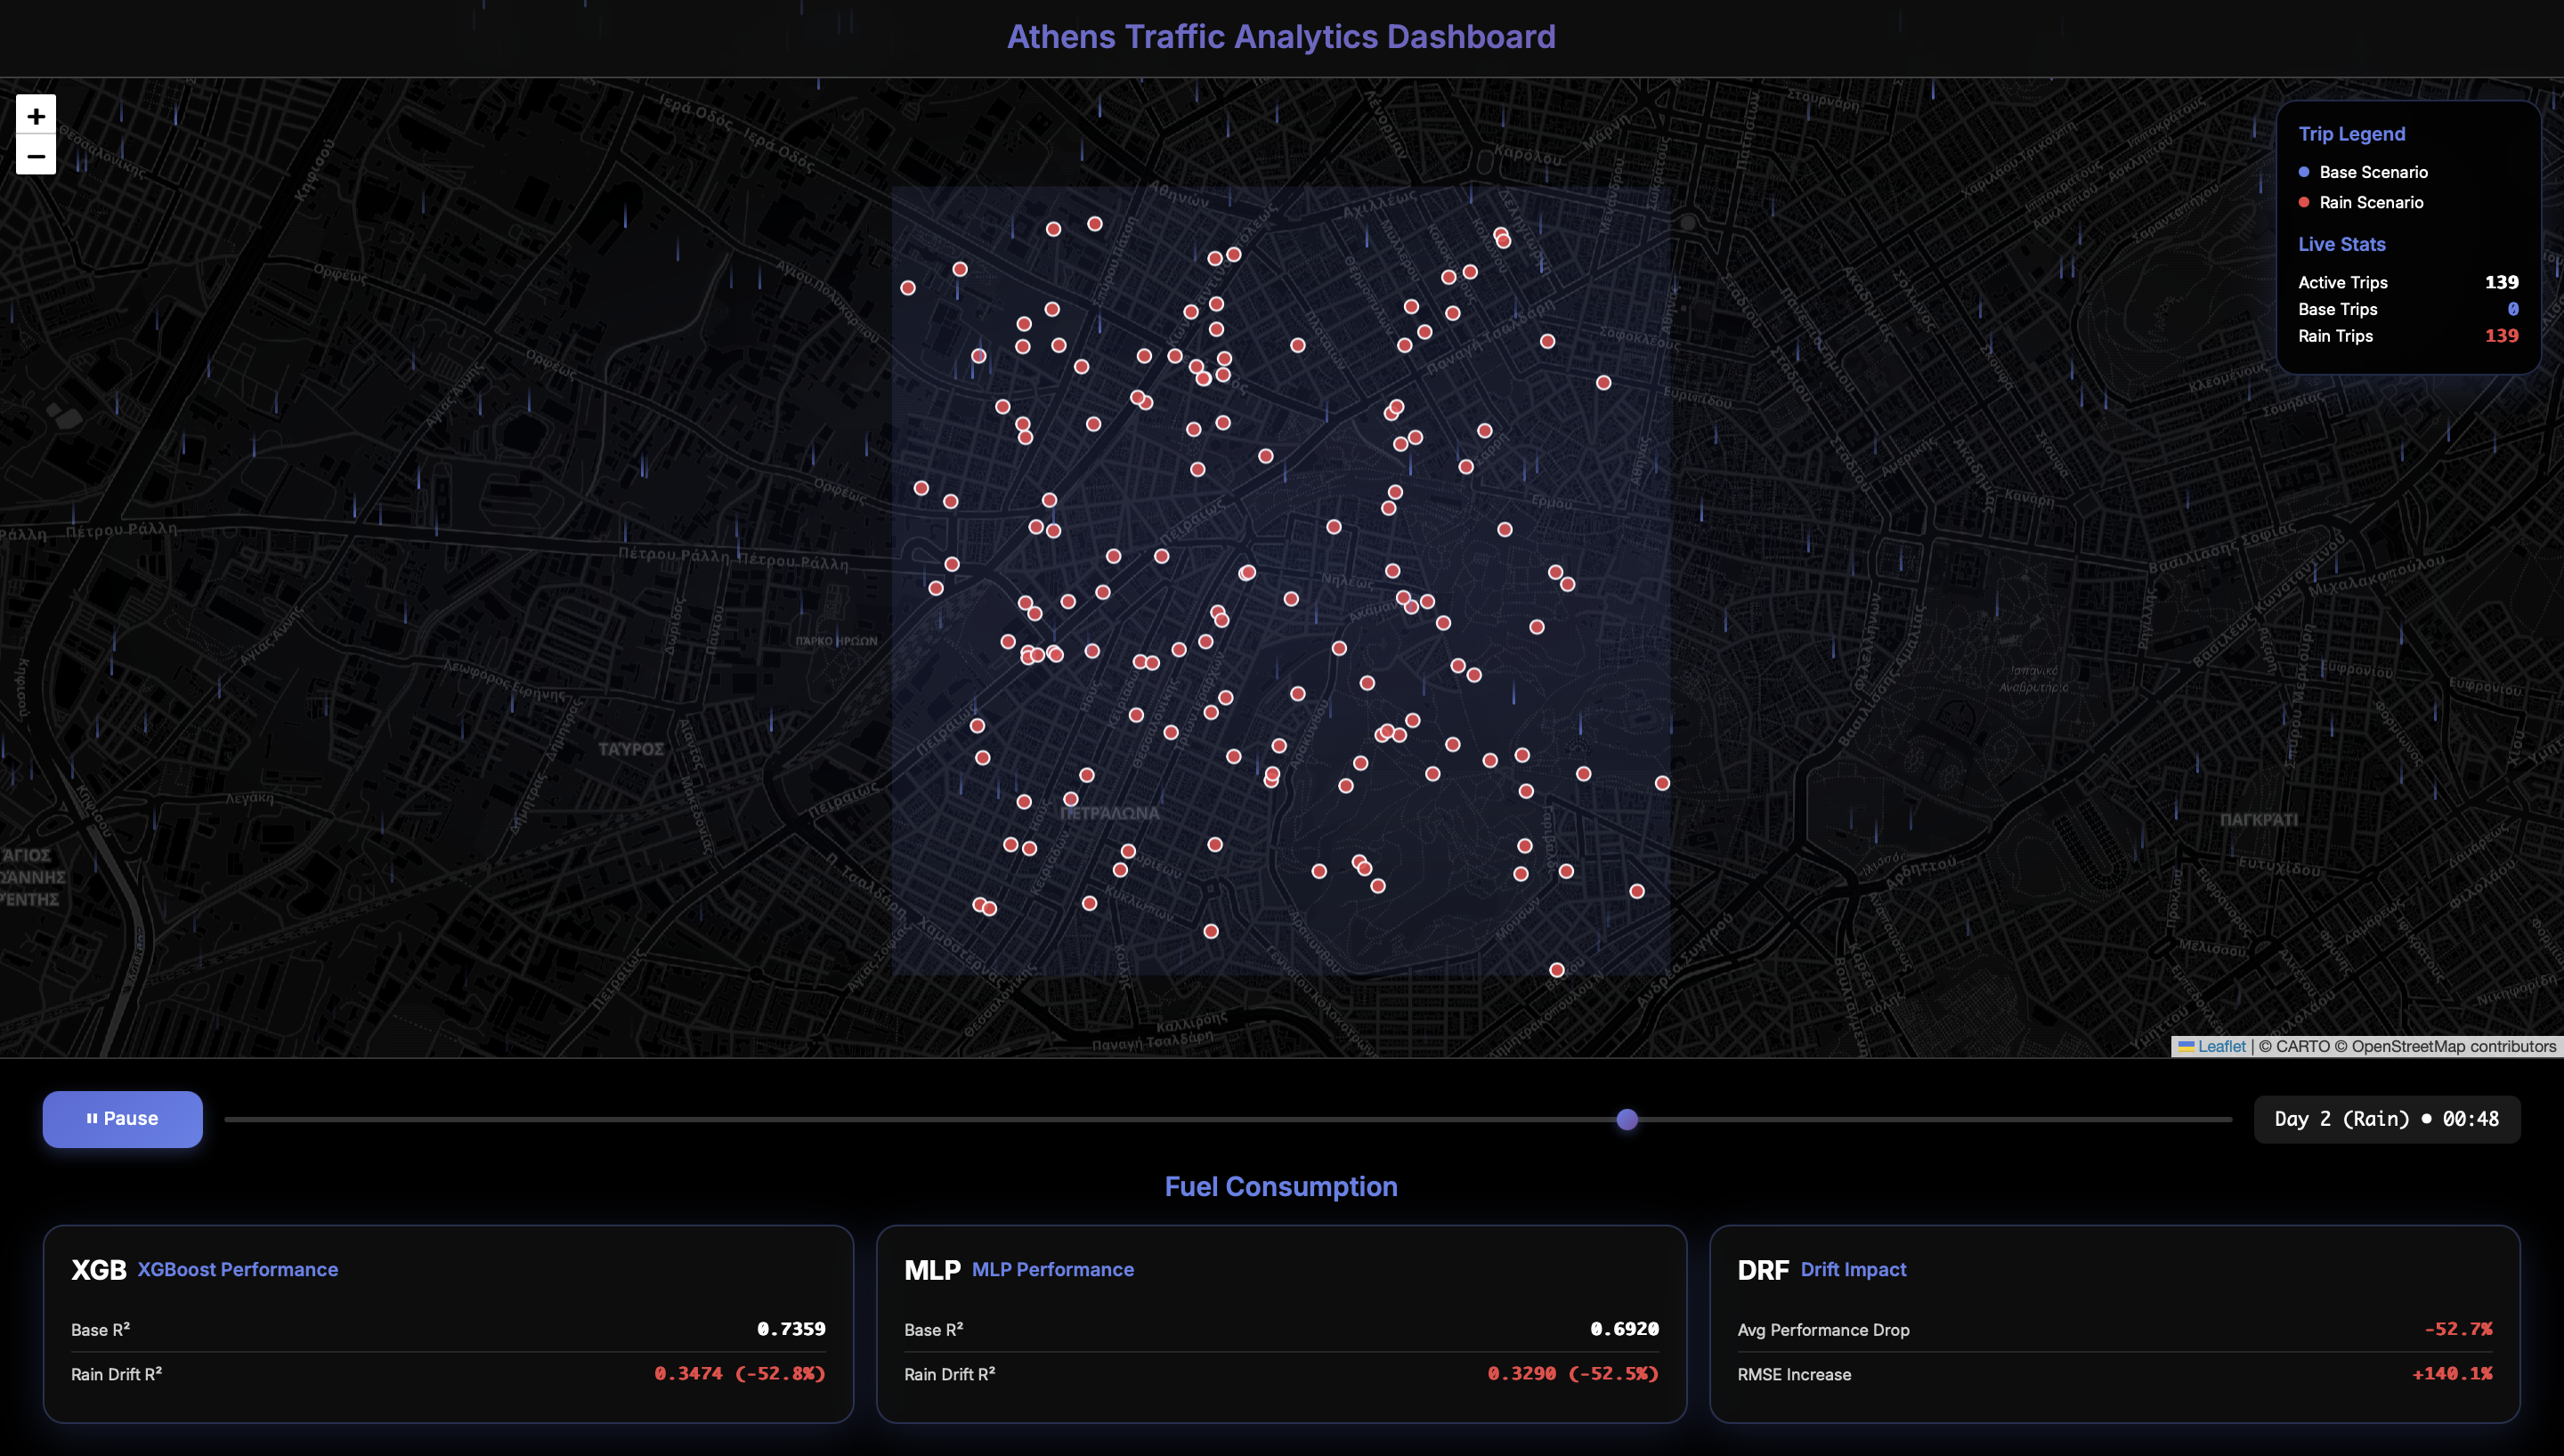
\includegraphics[width=0.6\textwidth]{figures/ui-mockup.png}
    \end{center}

    \begin{itemize}
        \item Static map with trip visualization
        \item Time-scrubber for simulation navigation
        \item Live statistics for base vs rain scenarios
    \end{itemize}
\end{frame}

\begin{frame}{Final User Experience Design}
    \begin{columns}[c]
        \column{0.5\textwidth}
        \begin{center}
            \textbf{Administrator Dashboard}\\
            \vspace{0.3em}
            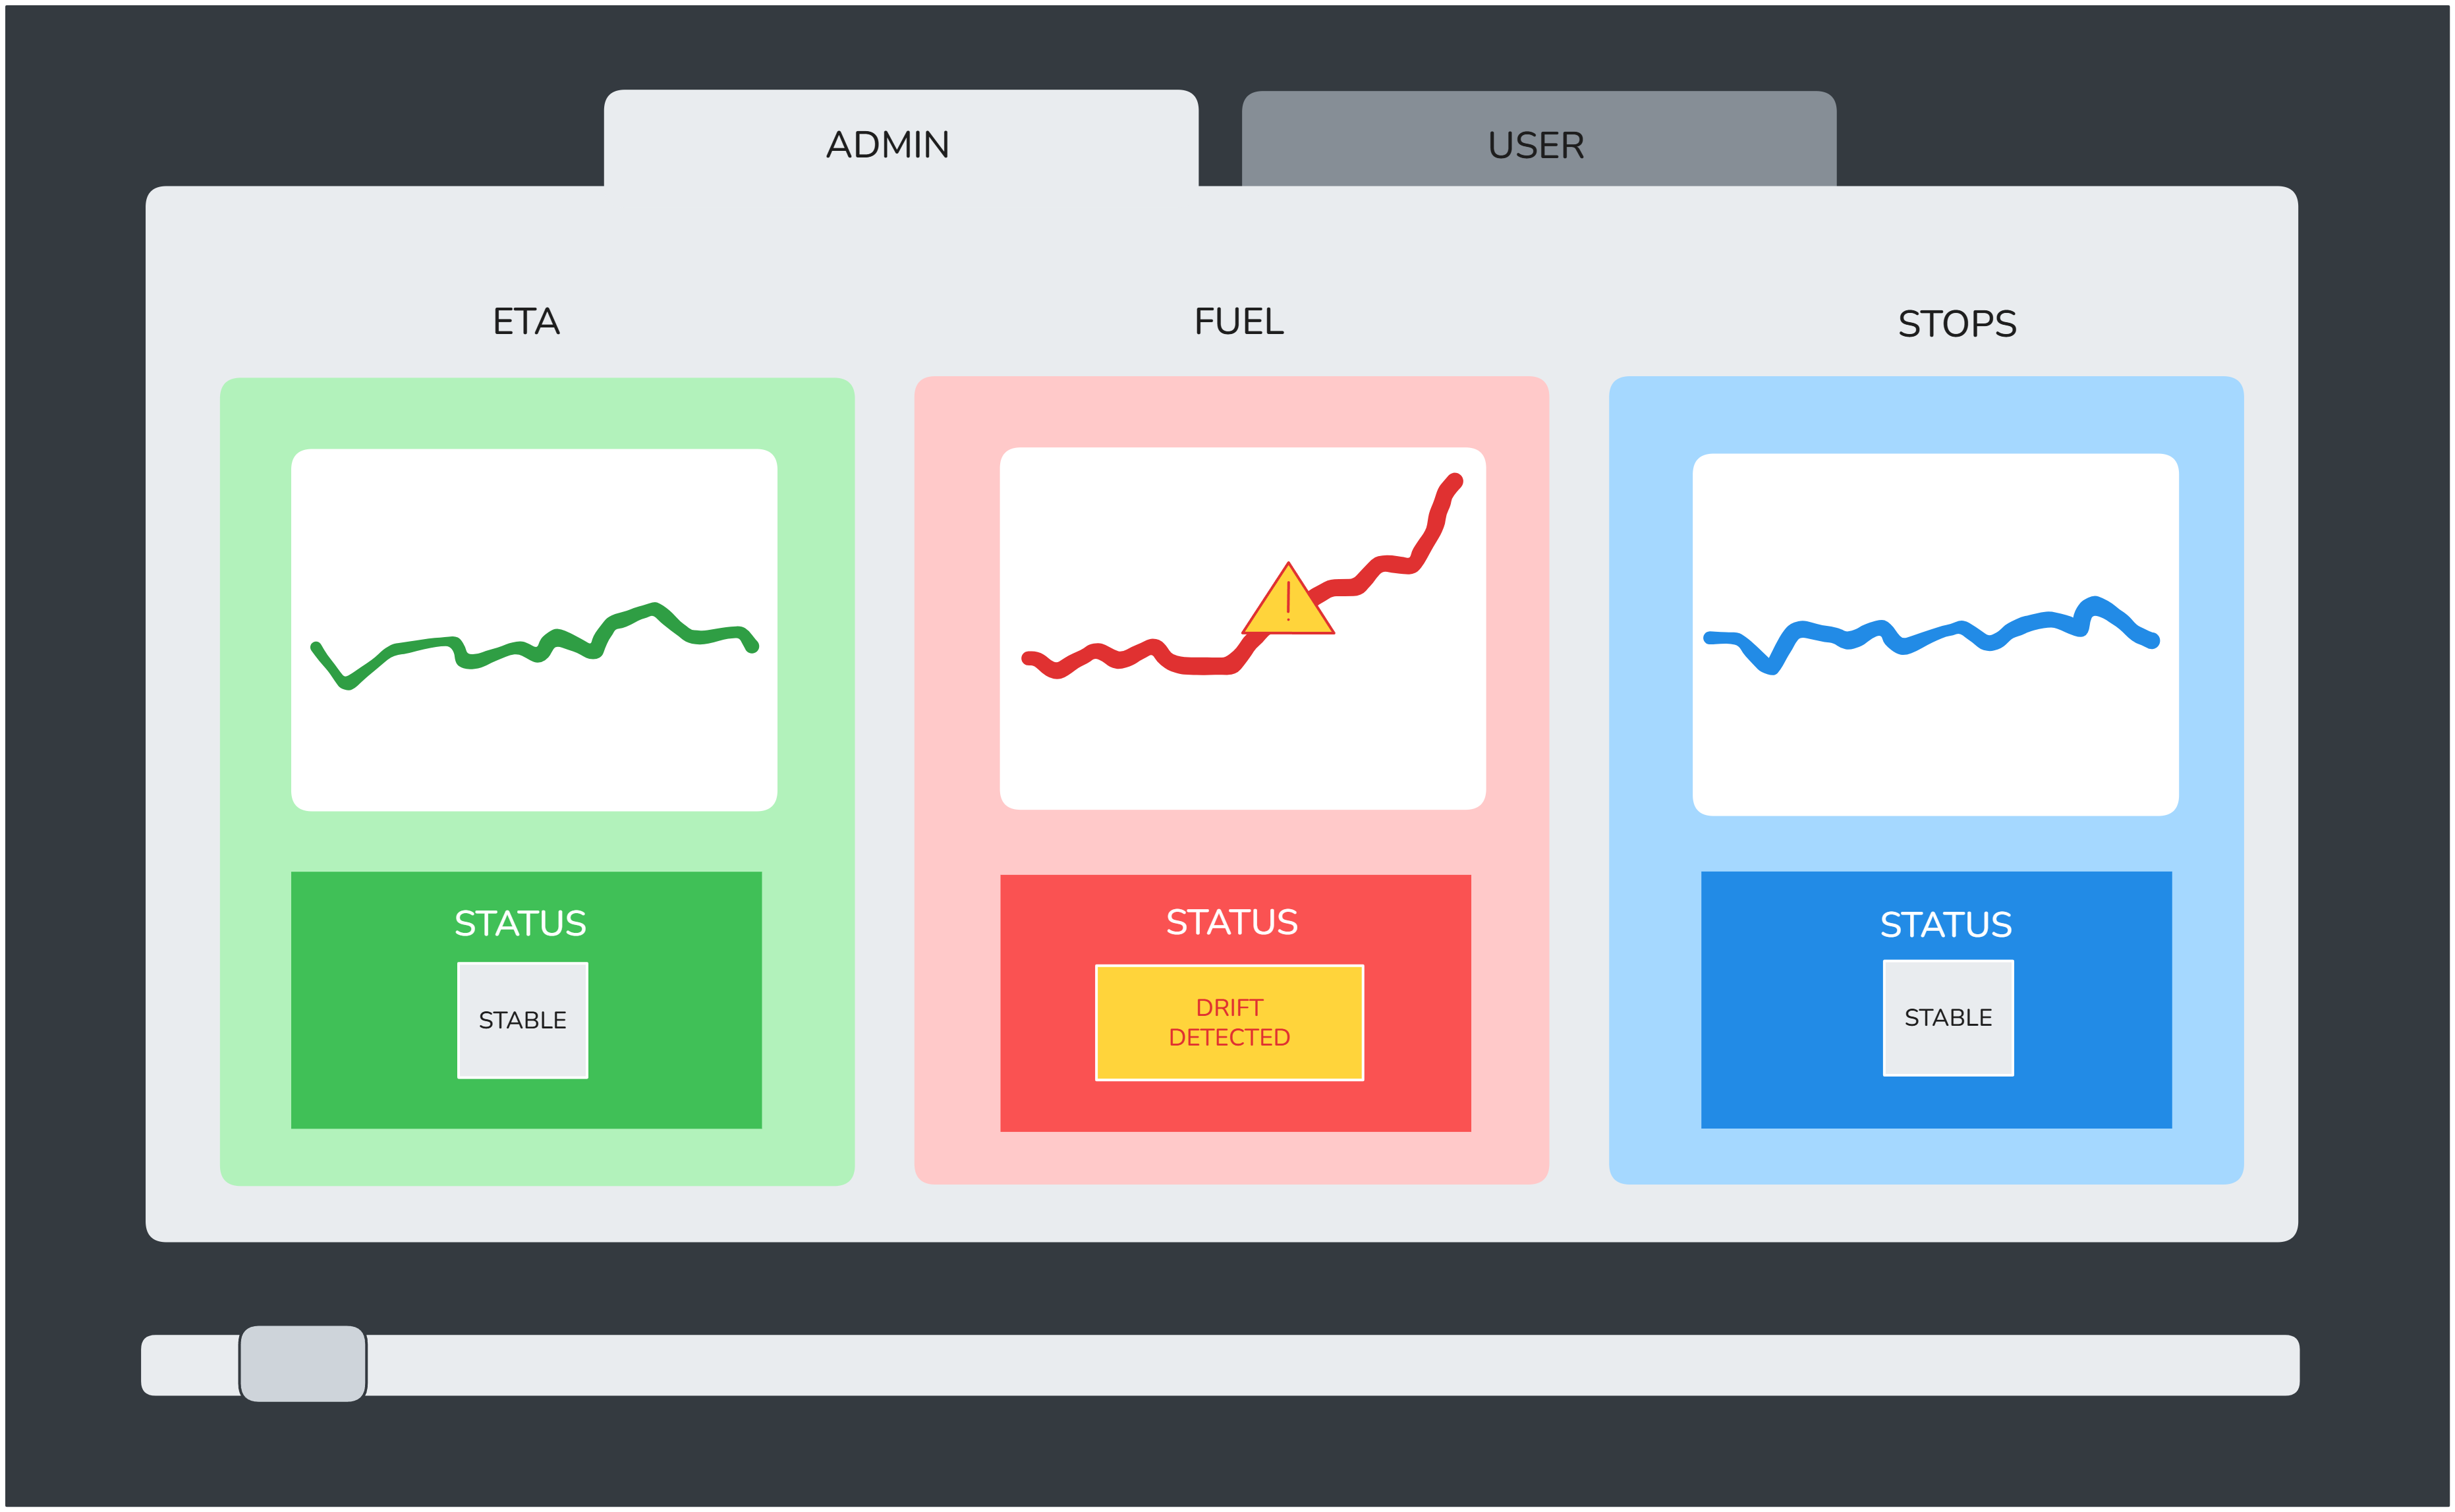
\includegraphics[width=\textwidth]{figures/admin-dashboard.png}
        \end{center}
        \begin{itemize}
            \item Time-series error visualization
            \item Multi-model monitoring
            \item Drift alerts \& retraining status
        \end{itemize}

        \column{0.5\textwidth}
        \begin{center}
            \textbf{User Interface}\\
            \vspace{0.3em}
            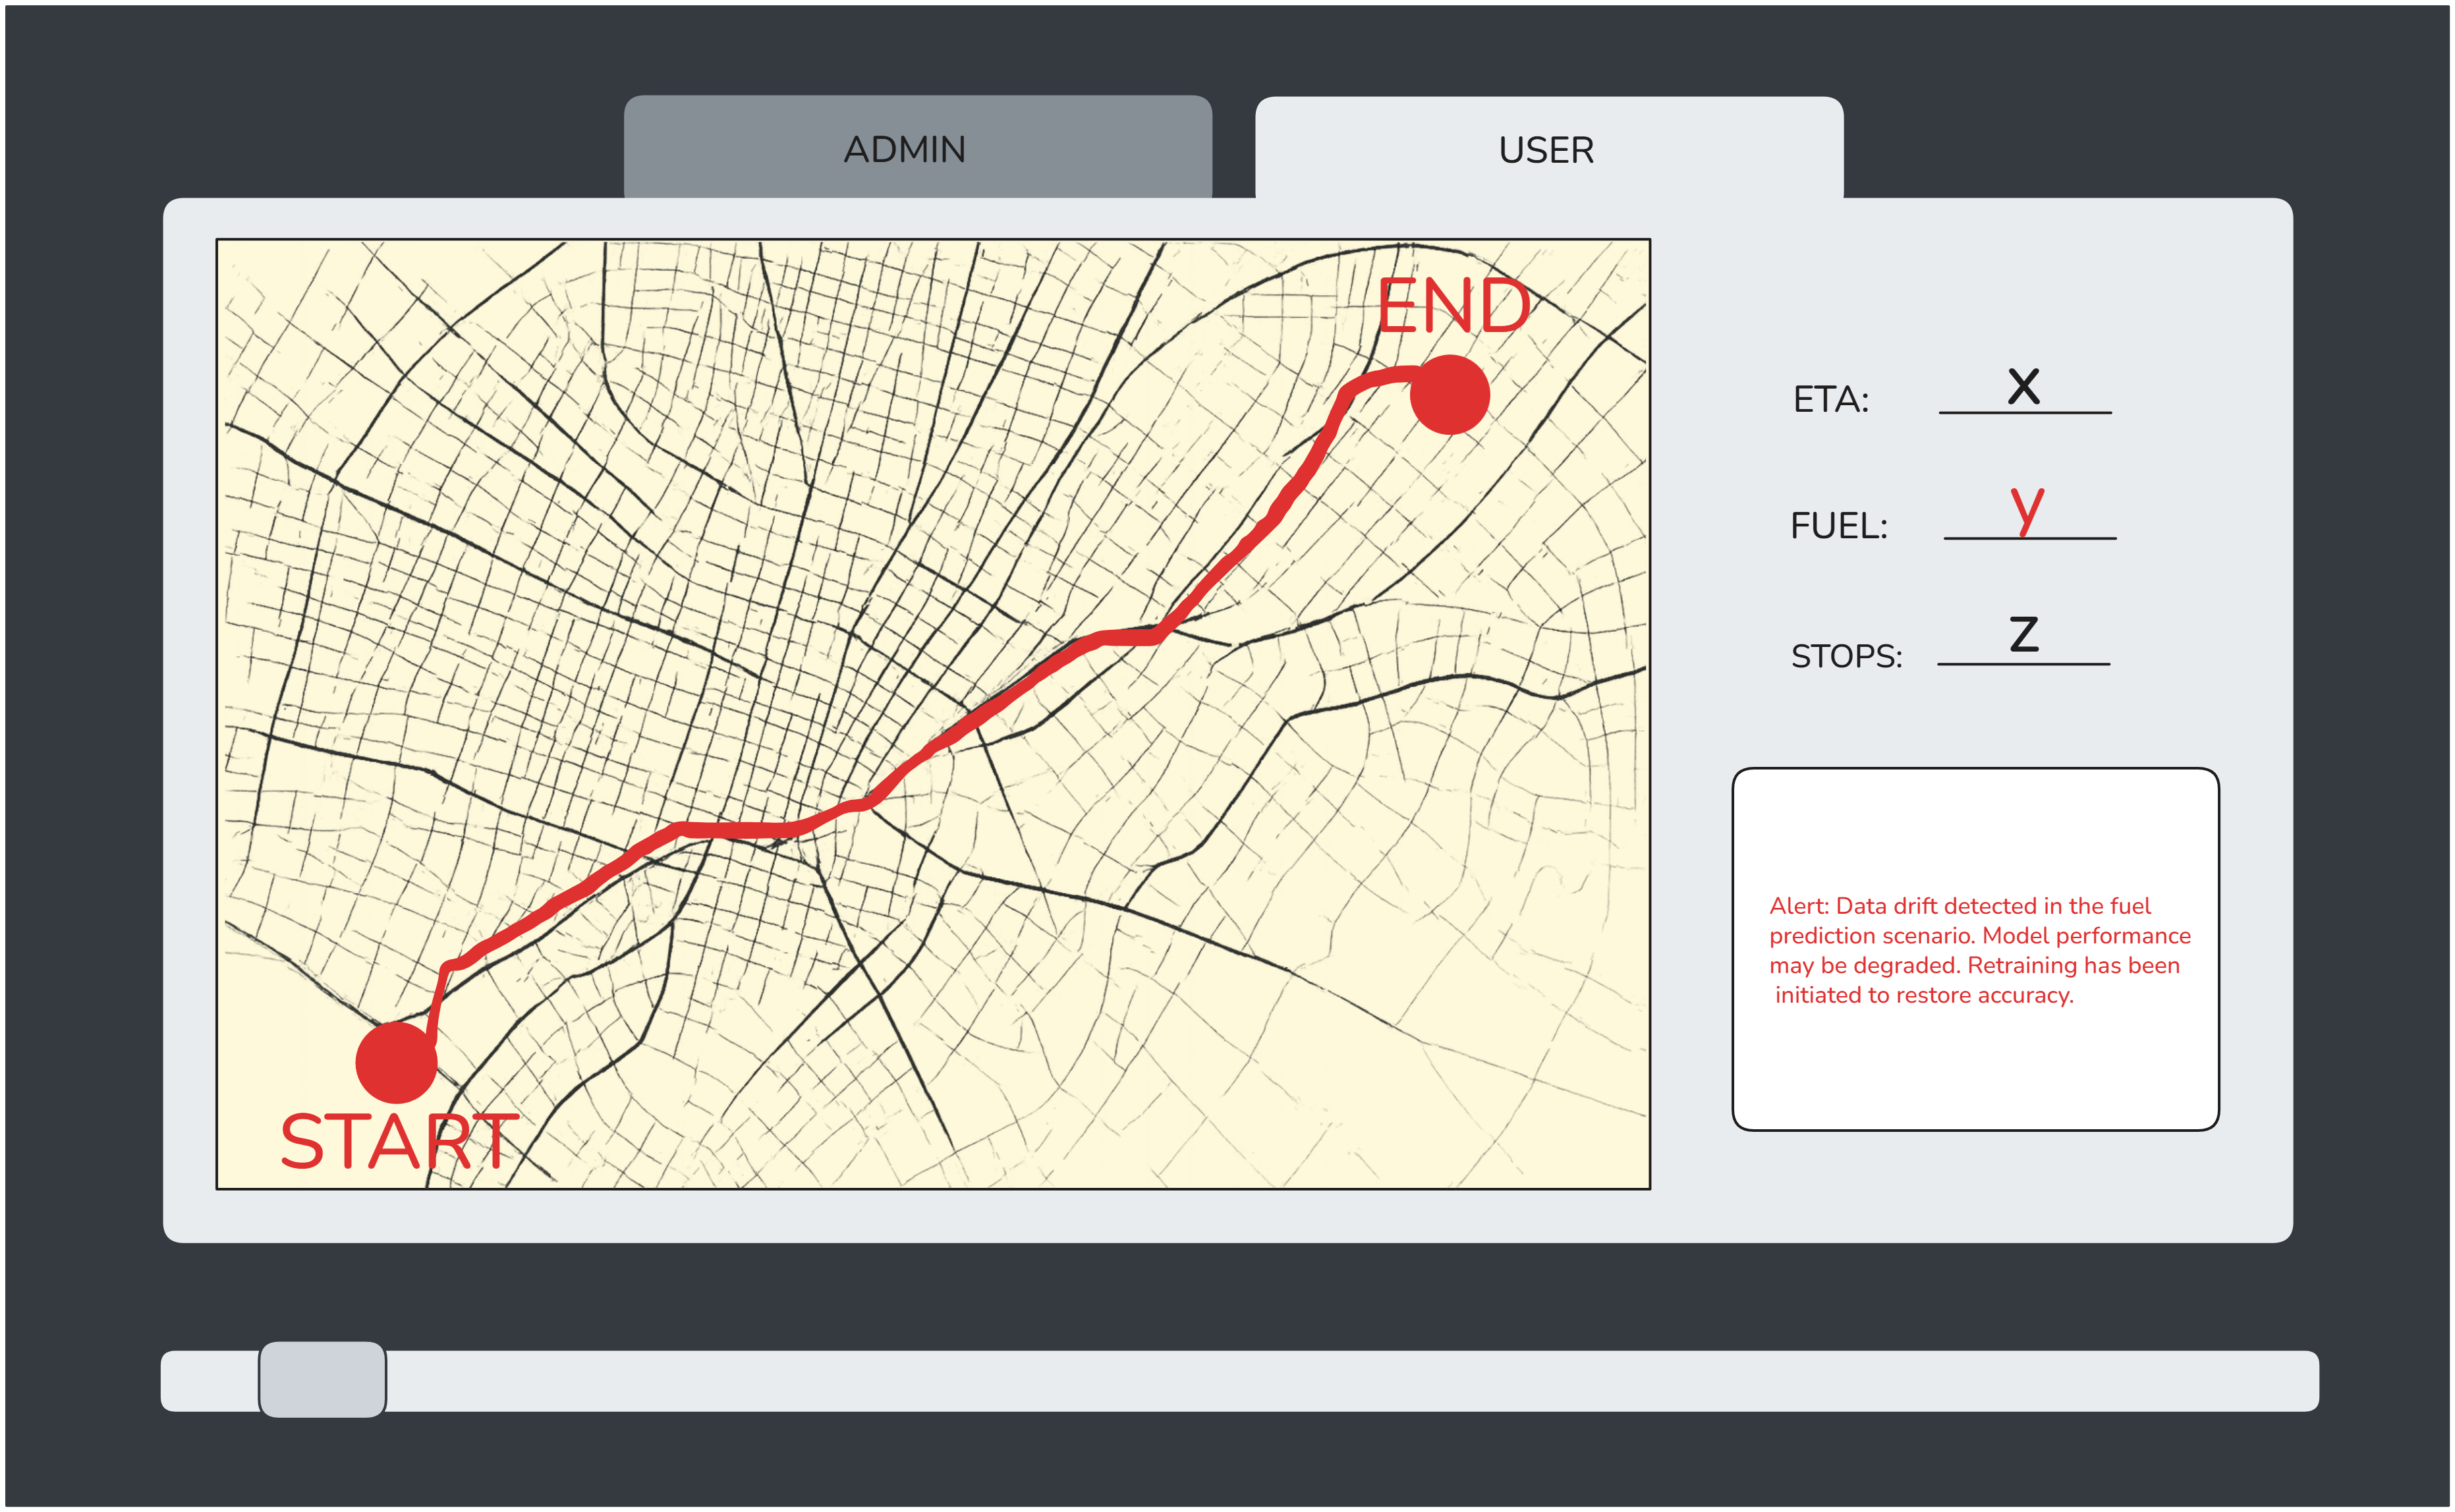
\includegraphics[width=\textwidth]{figures/user-interface.png}
        \end{center}
        \begin{itemize}
            \item Route selection \& visualization
            \item Real-time predictions
            \item Fuel, ETA, stops estimates
        \end{itemize}
    \end{columns}
\end{frame}

\begin{frame}{Platform Overview}
    \textbf{Goal}
    \begin{itemize}
        \item Run a time-lapse of a 20 h scenario (compressed to \(\sim\)4–5 min with 300x speedup).
        \item Continuously evaluate and monitor concept drift for three tasks: ETA, Fuel, Stops.
    \end{itemize}

    \textbf{Architecture}
    \begin{itemize}
        \item \textbf{Microservices} over HTTP/REST on a private \textbf{Docker} network, managed with \textbf{Docker Compose} and \textbf{uv} for dependencies.
        \item \textbf{Core technologies} include FastAPI, Pydantic, Dash, Plotly, River, and OpenAI.
        \item \textbf{Backend} as the orchestator - \textbf{Frontend} for the Admin Dashboard and the User Interface - \textbf{Predictor} for the batch/single inference and retraining - \textbf{Drift} for the concept drift monitoring - \textbf{Summarizer} for the AI-powered report generation.
    \end{itemize}
\end{frame}

\begin{frame}{Platform Architecture}
    \begin{figure}
        \centering
        
\includegraphics[width=0.72\textwidth]{figures/platform-architecture.png}
    \end{figure}
\end{frame}

\begin{frame}{Implementation Details}
    \textbf{Backend}
    \begin{itemize}
        \item Simulation timelapse driver (5 min simulated per tick), orchestration fan-out/fan-in, in-memory stores for metrics, notifications, and report.
        \item Task-agnostic design: windows in, predictions and errors out.
    \end{itemize}
    \textbf{Frontend}
    \begin{itemize}
        \item Admin Dashboard with simulation controls (start/pause/reset), live MAE charts, notifications, and report viewer.
        \item User Interface with Central Athens map, user O/D selection, route preview and on-demand multi-task predictions.
    \end{itemize}
    \textbf{Predictor ETA/Fuel/Stops}
    \begin{itemize}
        \item Parquet window data loader, and versioned model registry.
        \item Batch/single inference, error calculation and on-demand feature engineering.
        \item Background service for model retraining and interface with SUMO network for route preview and feature extraction.
    \end{itemize}
\end{frame}

\begin{frame}{Drift Detection Service Overview}

    \textbf{Role in the platform}
    \begin{itemize}
        \item Central service that monitors \textbf{model error streams} for all tasks (ETA, Fuel, Stops).
        \item Maintains \textbf{separate state per task} but applies a shared policy.
    \end{itemize}

    \vspace{0.4em}
    \textbf{Signal and smoothing}
    \begin{itemize}
        \item Uses rolling statistics on residuals to reduce noise before testing.
    \end{itemize}

    \vspace{0.4em}
    \textbf{Action on alarm}
    \begin{itemize}
        \item Emits a \textbf{drift event} to the orchestrator which triggers the \textbf{incremental retraining} process for the affected model and then \textbf{recalibrates} detectors.
    \end{itemize}

\end{frame}

\begin{frame}{Detectors \& Consensus Policy}

    \textbf{Detector ensemble}
    \begin{itemize}
        \item \textbf{ADWIN} (adaptive window) — abrupt mean shifts
        \item \textbf{Page–Hinkley} (CUSUM) — gradual mean changes
        \item \textbf{KSWIN} (K–S test) — general distribution shifts
        \item \textbf{SPC} (control limits) — persistent out-of-control behavior
    \end{itemize}

    \vspace{0.4em}
    \textbf{Consensus rule}
    \begin{itemize}
        \item Raise drift when \textbf{3 of 4} detectors agree within a short window.
        \item Design choice prioritizes \textbf{precision} (low false alarms) over speed.
    \end{itemize}

    \vspace{0.4em}
    \textbf{Time-critical variant}
    \begin{itemize}
        \item For faster response, relax consensus or favor abrupt-sensitive settings, accepting more false alarms.
    \end{itemize}

\end{frame}

\begin{frame}{Dynamic Calibration (Task-Agnostic)}

    \textbf{Why calibration}
    \begin{itemize}
        \item Each task has different error scale and variance.
        \item Fixed thresholds cause either missed drifts or false alarms.
    \end{itemize}

    \vspace{0.4em}
    \textbf{How it runs}
    \begin{itemize}
        \item Initial \textbf{grace period} on stable data to learn baseline error behavior.
        \item Auto-select \textbf{most sensitive non-firing} parameters per detector and per task.
    \end{itemize}

    \vspace{0.4em}
    \textbf{After adaptation}
    \begin{itemize}
        \item Re-run calibration on the new error regime to keep monitoring reliable.
    \end{itemize}

    \vspace{0.4em}
    \textbf{Outcome}
    \begin{itemize}
        \item \textbf{Task-agnostic} deployment with a single policy and manual tuning.
    \end{itemize}

\end{frame}

\begin{frame}{GenAI-Powered Automated Reporting}

    \textbf{Objective:} Convert simulation telemetry into human-readable summaries

    \vspace{0.4em}
    \begin{columns}[c]
        \column{0.55\textwidth}
        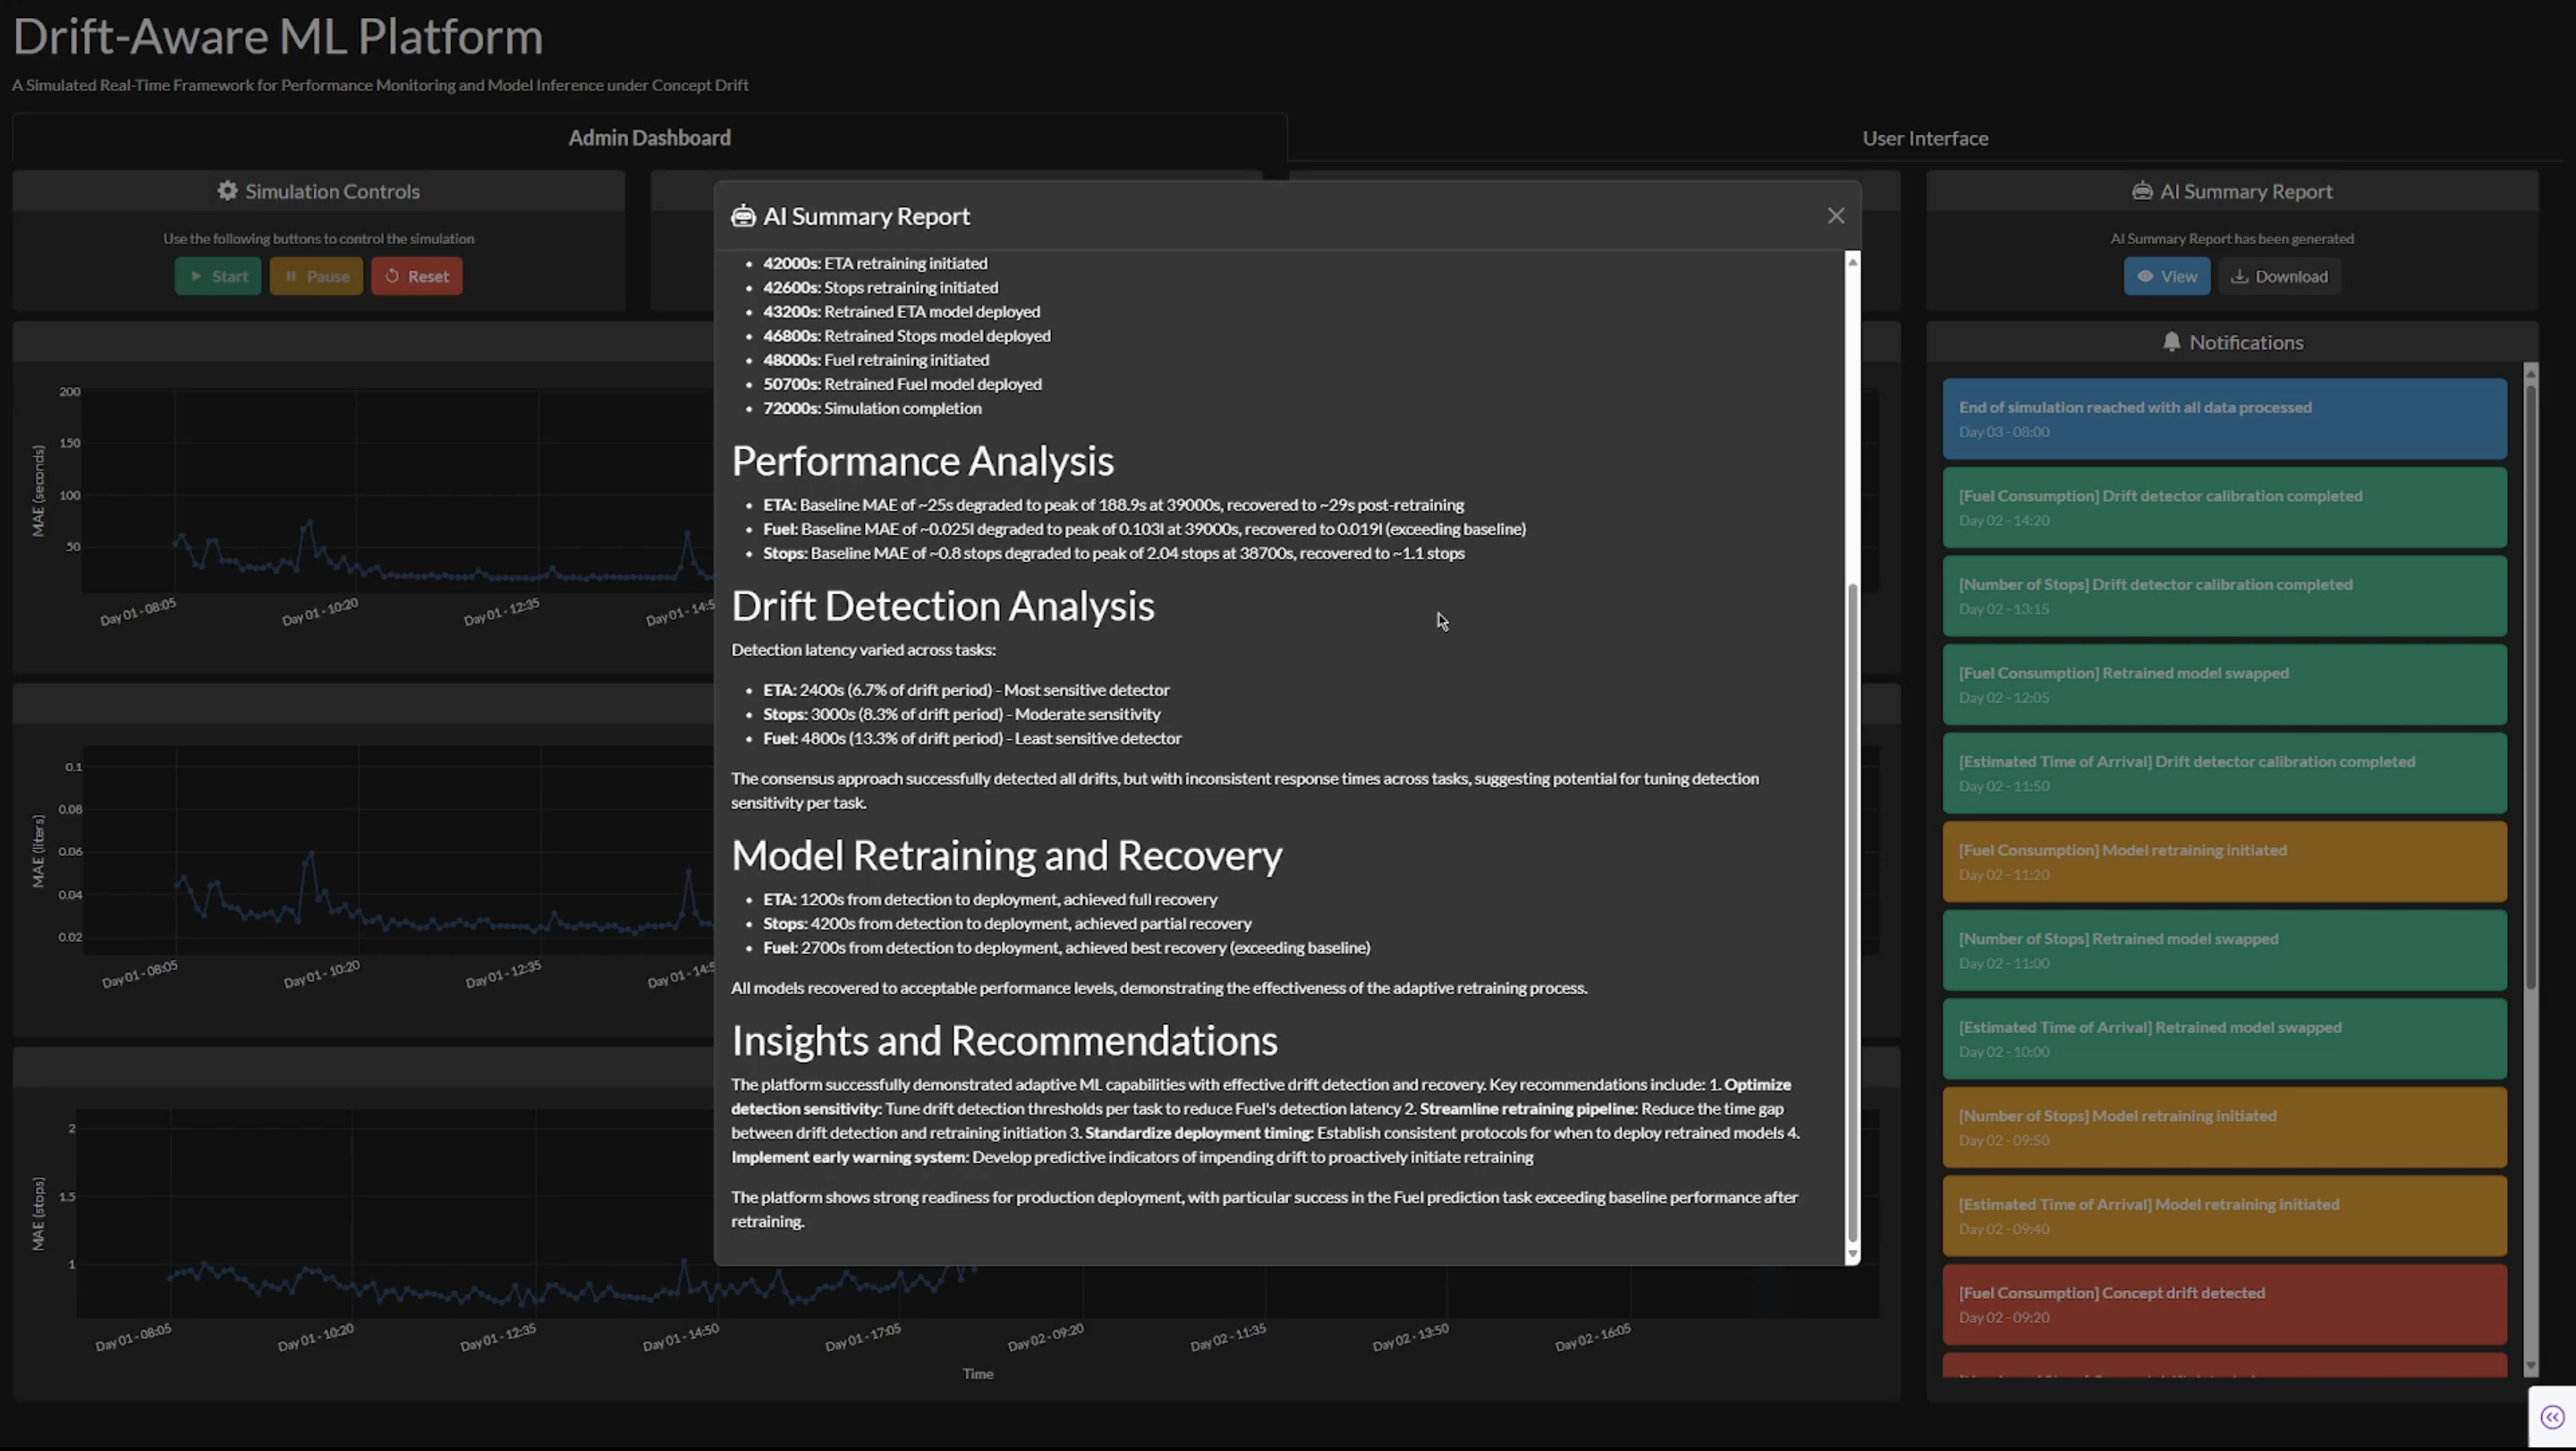
\includegraphics[width=\textwidth]{figures/platform-report.png}

        \column{0.43\textwidth}
        \textbf{Implementation:}
        \begin{itemize}
            \item LLM-based report generation
            \item Inputs: drift logs, MAE metrics, simulation events
            \item Output: Markdown $\rightarrow$ PDF
            \item GPT-4o (dev), glm-4.5-air (prod)
        \end{itemize}

        \vspace{0.4em}
        \textbf{Value Proposition:}
        \begin{itemize}
            \item Automated post-simulation docs
            \item Eliminates manual log analysis
            \item MLOps integration proof-of-concept
        \end{itemize}
    \end{columns}

\end{frame}

\begin{frame}{Platform Control Flow and Performance}
    \textbf{Per tick}
    \begin{itemize}
        \item Backend sends concurrent batch requests to predictors.
        \item Predictors infer, return errors/aggregates and the Backend forwards them to Drift.
        \item Drift updates detectors, returns state (Calibrating / Stable / Drifted / Retraining).
        \item If drifted: collect post-drift window → retrain → hot-swap → recalibrate.
        \item Frontend polls snapshots/metrics/notifications.
        \item Summarizer runs at completion to generate the AI-powered report.
    \end{itemize}

    \smallskip
    \textbf{Performance}
    \begin{itemize}
        \item Async I/O for fan-out/fan-in, CPU-bound work in separate processes (detectors updates, retrain), precomputed features in Parquet for batch speed and in-memory stores for hot loop.
        \item \textbf{Achieved:} about 300x scenario speed, interactive UI throughout.
    \end{itemize}
\end{frame}

\section{Results}

\begin{frame}{Platform Live Demo}
    \large Now we will go through a live demonstration of the platform, to see all the above in action!
\end{frame}

\begin{frame}{Platform Live Demo Takeaways}

    \begin{itemize}
        \item \textbf{Two 10-hour days} of data in a timelapse of \textbf{4-5 real time minutes}, the second one being with \textbf{rain conditions}.
        \item \textbf{Three} models (ETA, Fuel, Stops) evaluated on the data and \textbf{monitored for drift detection}.
        \item \textbf{Adaptation} of the above models, if drift is detected, and \textbf{hot-swap} of the new retrained models.
        \item \textbf{MAE charts} to visualize the progress of model errors over time.
        \item User Interface tab with the ability to request predictions for a \textbf{user input of origin/destination}.
        \item \textbf{AI-generated report} in the end of the simulation, including a summary.
    \end{itemize}

\end{frame}

\begin{frame}{Results}

    \textbf{Drift Detection}
    \medskip

    \begin{itemize}
        \item Zero false alarms on stable conditions
        \item Drift detected in 3/3 tasks
        \item Latency ranged from 40 minutes to 80 minutes
    \end{itemize}

    \medskip
    \textbf{Drift Adaptation}

    \begin{table}[htbp]
        \centering
        \caption{Impact of adaptation on model performance under drift conditions.}
        \label{tab:retraining_results}
        \small
        \begin{tabular}{lccc}
            \hline
            \textbf{Task} & \textbf{MAE - Baseline} & \textbf{MAE - Post Adaptation} & \textbf{Improvement} \\
            \hline
            ETA   & 43.27       & 32.27       & 25.4\% \\
            Fuel  & 17{,}517.13 & 17{,}077.28 & 2.5\% \\
            Stops & 1.149       & 0.898       & 21.9\% \\
            \hline
        \end{tabular}
    \end{table}

\end{frame}

\section{Conclusion}

\begin{frame}{Conclusion}
    \begin{itemize}

        \item We developed a \textbf{unified urban mobility platform} that continuously monitors, detects, and adapts to concept drift, while supporting multiple models.
        \item In the abrupt clear-to-rain scenario, the framework \textbf{detected drift} and \textbf{restored accuracy} through incremental retraining.
        \item The platform provides a foundation for \textbf{scalable, reliable deployment} in real urban environments.

    \end{itemize}
\end{frame}

\begin{frame}{Limitations and Future Work}
    \begin{itemize}
        \item \textbf{Synthetic data.} The evaluation is based on synthetic data generated through SUMO.
            \textbf{Next step:} Validate performance in real datasets of urban mobility.
            \medskip
        \item \textbf{Limited drift evaluation.} The platform is designed for multiple drift cycles but tested on a single abrupt case, without gradual or recurring drifts.
            \textbf{Next step:} Extend experiments to longer horizons with repeated, gradual, and incremental drift scenarios.
    \end{itemize}
\end{frame}

\begin{frame}{Questions}
    \centering
    \vfill
    {\large \textbf{Thank you for your time!}}\\[1em]
    {\large \textbf{Any questions?}}
    \vfill
\end{frame}

\end{document}
